
\chapter{Phonologically-conditioned allomorphy}
\section{Syllable-counting morphology in the plural}
\subsection{Regular words}

\subsubsection{old}
\footnote{This allomorphy is arbitrary and generally not phonologically-optimizing \citep{Vaux-2003-Syllabification}. Cross-linguistically, many cases of syllable-counting allomorphy are phonologically-optimizing and reference feet \citep{Kager-1996-AffixSyllableCounting,Gonzalez-2005-PhonoAllomorphyPanoan}. But, the Armenian allomorphy is not phonologically-optimizing. See \citet{Vaux-2003-Syllabification,Paster-2005-SubcatSyllableCounting,Paster-2006-PhonologicalConditionsAffixation,Paster-2019-PhonologyCounts} for more cases that do not reference feet and aren't optimizing.}


\subsection{Variation with final rising-sonority clusters}
\subsection{Morphologically-induced variation}
\subsection{Compounds}
Summarize and refer people to compounding chapter
"b)	"

նախասիրտ and semantics. got pl as er even though meaning isnt technically heart

\section{Syllable-counting morphology in the plural possessive}
\section{Syllable-counting morphology in the indicative}
\section{Vowel-consonant conditions in the definite and indefinite}



\chapter{Lexical phonology and strata}

also mention here that we talked about passive being funny a lot. ideally a list of all the funny morphophon phenomena and their interactions

can take picture of trees from nllt paper maybe

maybe have a passive seection
\section{old}

\subsection{nllt high vowel}
\subsubsection{nlltformalization}
I formalize the above derivation vs.\ inflection distinction with stem vs.\ word strata \citep{Kiparsky-1982-lexicalMorphoPhono,Kiparsky-2000-OpacityCyclicity,Kiparsky-2015-StratalOT,Bermudez-2011-Cyclicity,Bermudez-2012-ArchitectureDivisionLaborExponence,BermudezOtero-2018-StratalPhonology}. Free-standing roots, derivational suffixes, and compounds form Morphological Stems (MStems or MS), while inflection creates Morphological Words (MWords or MW). MStems trigger the stem-level cophonology of stress and DHR; MWords trigger the word-level cophonology of stress without reduction. I illustrate the stratal derivation of the base \textit{\textipa{ɑmusin}}, its derivative \textit{\textipa{ɑmusn-utjun}}, and its inflected form \textit{\textipa{ɑmusin-ov}}. 


\begin{exe}
	
	\ex \textit{Stratal derivation of the root} \textipa{ɑmusin}, \textit{derivative} \textipa{ɑmusn-utjun}, \textit{and inflected} \textipa{ɑmusin-ov}\label{nlttPaperderivation table: WA amusin amusinov amusinner}\\
	
	\hspace*{-1cm}\resizebox{1\textwidth}{!}{%
		\begin{tabular}{||llll | lll||}
			\hline
			&&&&
			\begin{tikzpicture}[scale = 0.8]
				
				\Tree [.MW_{\textsc{nom}} [.MS_{\textit{n}} [.$\sqrt{}$ /\textipa{ɑmusin}/ ] [.\textit{n} -$\emptyset$ ] ] [ [.\textsc{nom} -$\emptyset$ ] ] ] 
				
			\end{tikzpicture} 
			&
			\begin{tikzpicture}[scale = 0.8]
				
				\Tree [.MW_{\textsc{nom}} [.{MS}_{\textit{n}} [.MS_{\textit{n}} [.$\sqrt{}$ /\textipa{ɑmusin}/ ] [.n -$\emptyset$ ] ] [ [.\textit{n} /\textipa{-utjun}/ ] ] ] [ [ [.\textsc{nom} -$\emptyset$ ] ] ] ]
				
				
			\end{tikzpicture} 
			&
			\begin{tikzpicture}[scale = 0.8]
				
				\Tree [.MW_{{\ins}} [.MS_{\textit{n}} [.$\sqrt{}$ /\textipa{ɑmusin}/ ] [.\textit{n} -$\emptyset$ ] ] [ [.{\ins} /-\textipa{ov}/ ] ] ]
				
			\end{tikzpicture} 
			\\
			Input &&& & \textipa{/amusin -$\emptyset$_S -$\emptyset$_W /} & \textipa{/amusin -$\emptyset$_S -utjun_S -$\emptyset$_W/} & \textipa{/amusin -$\emptyset$_S -ov_W/} \\\hline\hline
			\textit{Cycle 1} & \textsc{Morph}&&Spell-out & \textipa{/amusin -$\emptyset$_S /} & \textipa{/amusin -$\emptyset$_S/} & \textipa{/amusin -$\emptyset$_S/} \\
			% & \textsc{Prosody}&&Syllabify & \textipa{ɑmusin} &\textipa{ɑmusin} &\textipa{ɑmusin} \\
			& \textsc{Phono}&\textit{SLevel} & Stress & \textipa{ɑmus\'in} &\textipa{ɑmus\'in} &\textipa{ɑmus\'in} \\
			&&&DHR & && \\
			\hline
			\textit{Cycle 2}&\textsc{Morph}&& Spell-out & \cellcolor{lightgray} & \textipa{ɑmus\'in - /-utjun_S}/ &\cellcolor{lightgray} \\
			% &\textsc{Prosody}& &Syllabify & \cellcolor{lightgray} & \textipa{ɑmus\'in-utjun} & \cellcolor{lightgray} \\
			& \textsc{Phono}& \textit{SLevel} & Stress & \cellcolor{lightgray} &\textipa{ɑmus\v{i}n-utj\'un} &\cellcolor{lightgray} \\
			&& &DHR & \cellcolor{lightgray} &\textipa{ɑmusn-utj\'un}&\cellcolor{lightgray} \\
			\hline
			\textit{Cycle 3} &\textsc{Morph}&&Spell-out&\textipa{ɑmus\'in /-$\emptyset$_W/} &\textipa{ɑmusn-utj\'un /-$\emptyset$_W/}& \textipa{ɑmus\'in /-ov_W/}\\
			% &\textsc{Prosody}&&Syllabify& && \textipa{ɑmus\'in-ov}\\
			& \textsc{Phono}&\textit{WLevel}& Stress& \textipa{ɑmus\'in} & \textipa{ɑmusn-utj\'un}& \textipa{ɑmus\v{i}n-\'ov}\\
			\hline\hline
			Output&&& &\textipa{ɑmus\'in} & \textipa{ɑmusn-utj\'un} & \textipa{ɑmusin-\'ov}\\
			\hline 
		\end{tabular}
	}
\end{exe}


Each cycle includes a round of morphological, and phonological processes. The phonological processes are triggered by different cophonologies \citep{Inkelas-2014-Interplay}. The MStems and MWords have a subscript for their morphosyntactic feature. In their underlying form, affixes have a subscript \textit{_S} or \textit{_W} to indicate that they trigger the stem-level or word-level cophonology. I assume that free-standing roots form an MStem with a covert category-head \citep{Giegerich-1999-LexicalStrataEnglish,Marantz-2007-PhasesWords}. I assume that stems can form MWords via covert nominative case. Grey cells indicate that a given item doesn't undergo a certain step. 













In Cycle 1, the root is spelled out, syllabified, and undergoes the stem-level phonology to get stressed: \textit{\textipa{ɑmus\'in}}. In Cycle 2, the derivative is formed. The stem-level phonology of stress shift and reduction is applied: \textit{\textipa{ɑmusn-utj\'un}}. In Cycle 3, covert or overt inflection is added and the word-level cophonology is applied. For the base and derivative, Cycle 3 vacuously places stress on the last syllable again. For the inflected word \textit{\textipa{ɑmusin-ov}}, the word-level phonology is applied with stress shift but no reduction: \textit{\textipa{ɑmusin-\'ov}}. I assume that the word-level is postcyclic, and that the stem-level is cyclic \citep{BooijRubach-1987-PostcyclicPostLexical}. %In the next section, I provide additional evidence for strata in Western Armenian.% in S\ref{nlttPapersection: reduction: strata elsewhere in WA}.



Below, I illustrate the relevant re-rankings to trigger DHR in the stem-level for \textit{\textipa{ɑmusn-utj\'un}}, but block it in the word-level for \textit{\textipa{ɑmusin-\'ov}}.% The faithfulness constraints (in bold) are low-ranked in the stem-level tableau (\ref{nlttPaperot table dhr stem}), and high-ranked in the word-level tableau (\ref{nlttPaperot table dhr word}).





\begin{exe}
	\ex 
	\begin{multicols}{2}
		
		\begin{xlist}
			
			\ex ~\label{nlttPaperot table dhr stem}\\
			
			\vspace{-.9cm}\hspace*{-2cm} \renewcommand*\arraystretch{1.2}
			\scalebox{1}[1]{\begin{tabular}[t]{|rrl||c|c|c|} \hline
					\multicolumn{3}{|c||}{\textipa{[amus\'in] + /-utjun/}} & *\textit{\v{i},\v{u}} & \textbf{\textsc{ Id[f]} }& \textbf{\textsc{Max-V} }\\[0.5ex]
					\hline a. & & \textipa{ɑmus\v{i}n-utj\'un} & $\ast$! & \cellcolor{lightgray} & \cellcolor{lightgray} \\
					\hline b. & \ding{43} & \textipa{ɑmusn-utj\'un} & & & \cellcolor{lightgray}$\ast$ \\
					\hline c. & & \textipa{ɑmus@n-utj\'un} & & $\ast$! & \cellcolor{lightgray} \\
					\hline \end{tabular}} \renewcommand*\arraystretch{1} 
			
			
			
			
			\ex ~\label{nlttPaperot table dhr word}\\
			
			\vspace{-1cm}
			\hspace*{-1cm} \renewcommand*\arraystretch{1.2}
			\scalebox{1}[1]{\begin{tabular}[t]{|rrl||c:c|c|} \hline
					\multicolumn{3}{|c||}{\textipa{[amus\'in] + /-ov/}} & \textbf{\textsc{ Id[f]}} & \textbf{\textsc{Max-V} }& *\textit{\v{i},\v{u}} \\[0.5ex]
					\hline a. & \ding{43} & \textipa{ɑmus\v{i}n-\'ov} & & & \cellcolor{lightgray}$\ast$ \\
					\hline b. & & \textipa{ɑmusn-\'ov} & & $\ast$! & \cellcolor{lightgray} \\
					\hline c. & & \textipa{ɑmus@n-\'ov} & $\ast$! & & \cellcolor{lightgray} \\
					\hline \end{tabular}} \renewcommand*\arraystretch{1} 
		\end{xlist}
	\end{multicols}
\end{exe}

In the stem-level (\ref{nlttPaperot table dhr stem}), the faithfulness constraints {\textsc{ Id[f]}},{\textsc{Max-V}} (in bold) are outranked by the output constraint *\textit{\v{i},\v{u}}. As explained in S\ref{nlttPapersection: reduction: destressed high reduction WA: organization: DEE}, this ranking triggers destressed high vowel reduction. In contrast in the word-level (\ref{nlttPaperot table dhr word}), these faithfulness constraints are promoted above the output constraint. This blocks high vowel reduction in the word-level.


% The next section examines DHR more closely. I show that it is cyclic (S\ref{nlttPapersection: reduction: destressed high reduction WA: organization: cyclic}). Exceptions and variation in DHR exist but they support the stratal model (S\ref{nlttPapersection: reduction: variation: der}, \ref{nlttPapersection: reduction: destressed high reduction WA: inflection overapply}). 


% For the compound \textit{\textipa{ɑmusn-a-zurg}} (\ref{nlttPaperexample: DHR in WArm domains}b-iii), its derivation is in (\ref{nlttPaperderivation table: WA compound amusnazurg}). The two individual stems undergo their own stem-level cycles. They are concatenated to form a single larger MStem and undergo the stem-level cophonology again. The linking vowel \textit{-a-} is a zero-morph that is inserted in spell-out. 


% \begin{exe}
	% \ex Stratal derivation of the compound \textit{\textipa{ɑmusn-a-zurg}} (\ref{nlttPaperexample: DHR in WArm domains}b-iii)\label{nlttPaperderivation table: WA compound amusnazurg}
	% \begin{center}
		% \begin{tabular}{||llll | l||}
			% \hline
			
			% &&&&
			
			% \begin{tikzpicture}[scale = 0.8]
				
				% 		\Tree [.a_S [.n_S [.$\sqrt{}$ /\textipa{ɑmusin}/ ] [.n -$\emptyset$ ] ] [.a_S [.$\sqrt{}$ /\textipa{zurg}/ ] [.a -$\emptyset$ ] ] ]
				
				% 		\end{tikzpicture} 
			
			% \\
			% Input & && &\makebox[2cm][l]{\textipa{/amusin -$\emptyset$_S}} + \textipa{/zurg -$\emptyset$/} \\\hline\hline
			% SLevel &Cycle 1& \textsc{Morph}&Spell-out & \makebox[2cm][l]{\textipa{/amusin -$\emptyset$_S/}} \textipa{/zurg -$\emptyset$_S/} \\
			% && \textsc{Struc}&Syllabify & \makebox[2cm][l]{\textipa{ɑ.mu.sin}} \textipa{zurg} \\
			
			% && \textsc{Phono}&Stress & \makebox[2cm][l]{\textipa{ɑ.mu.s\'in}} \textipa{z\'urg} \\
			% &&& DHR & \\
			% \hline
			% SLevel &Cycle 2& \textsc{Morph}&Compound & \makebox[1.7cm][l]{\textipa{ɑ.mu.s\'in}} \textipa{-a- z\'urg} \\
			% && \textsc{Struc}&Syllabify &\textipa{ɑ.mu.s\'i.n-a-z\'urg} \\
			% && \textsc{Phono}&Stress &\textipa{ɑ.mu.s\v{i}.n-a-z\'urg} \\
			% &&& DHR &\textipa{ɑ.mus.n-a-z\'urg} \\
			% \hline\hline
			% WLevel &&\textsc{Morph}&Spell-out&\textipa{ɑmusn-a-z\'urg} \\
			% &&Stress&& \\
			% \hline\hline
			% Output&&& &\textipa{ɑmusn-a-z\'urg} \\
			% \hline 
			% \end{tabular}
		
		% \end{center}
	% \end{exe}



% \subsubsection{Inflection and vowel reduction}\label{nlttPapersection: reduction: destressed high reduction WA: inflection overapply}










% \begin{exe}
	% \ex 
	% \begin{multicols}{3}
		% \begin{xlist}
			
			% \ex \makebox[2cm][l]{\textipa{S\'un-@}}`his/the dog'\label{nlttPaperexample: poss sing C}\\
			% \makebox[2cm][l]{\textipa{S\'un-@s}}`my dog'\\
			% \makebox[2cm][l]{\textipa{S\'un-@t}}`your.\textsc{sg} dog ' 
			% \ex \makebox[2cm][l]{\textipa{gad\'u-n}}`his/the cat\label{nlttPaperexample: poss sing V}\\
			% \makebox[2cm][l]{\textipa{gad\'u-s}}`my cat'\\
			% \makebox[2cm][l]{\textipa{gad\'u-t}}`your.\textsc{sg} cat ' 
			% \ex \makebox[2.44cm][l]{\textipa{Sun-er-n\'i-s}}\text{`our dog(s)'}\label{nlttPaperexample: plural poss}\\
			% \makebox[2.4cm][l]{\textipa{ɑx\t{tS}ig-n\'i-s}}`our girl'\\
			% \makebox[2.4cm][l]{\textipa{ɑx\t{tS}ig-ner-n\'i-s}}\text{`our girls'}
			% \end{xlist}
		
		
		% \end{multicols}
	
	% \end{exe}




% % \begin{exe}
	% % \ex 
	% % \begin{multicols}{2}
		% % \begin{xlist}
			
			% % \ex \makebox[2cm][l]{\textipa{k\'ir}}`writing (n)'\label{nlttPaperexample: verb base}\\
			% % \makebox[2cm][l]{\textipa{k@r-\'e-l}}`to write (root-\textsc{th}-\textsc{inf})' \\
			% % \ex \makebox[2cm][l]{\textipa{k@r-\'e-m}}`I write (root-\textsc{th}-\textsc{1sgPst})\label{nlttPaperexample: verb infl}'\\
			% % \makebox[2cm][l]{\textipa{k@r-\'e-t͡s-i}}`\text{I wrote (root-\textsc{th}-\textsc{aor}-\textsc{1sgPast})' }
			% % \ex \makebox[2cm][l]{\textipa{k@r-\'ɑd͡z}}`written (root-\textsc{prtp})'\label{nlttPaperexample: verb part} 
			
			
			% % \end{xlist}
		
		% % \end{multicols}
	% % \end{exe}

% To summarize, in Western Armenian, DHR is triggered in derivation but robustly blocked in inflection.
\subsubsection{diss:Destressed High Vowel Reduction  in Western Armenian}\label{disssection: reduction: destressed high reduction WA}










I formalize the above derivation vs.\ inflection distinction   with   stem vs.\ word strata \citep{Kiparsky-1982-lexicalMorphoPhono,Kiparsky-2000-OpacityCyclicity,Kiparsky-2015-StratalOT,Bermudez-2011-Cyclicity,Bermudez-2012-ArchitectureDivisionLaborExponence,BermudezOtero-2018-StratalPhonology}.  Free-standing roots, derivational suffixes, and compounds form    Morphological Stems (MStems or MS), while inflection creates Morphological Words (MWords or MW). MStems trigger the stem-level cophonology of stress and DHR; MWords trigger the word-level cophonology of stress without reduction. 
In (\ref{dissderivation table: WA amusin amusinov amusinner}), I illustrate the stratal derivation  of the base \textit{\textipa{ɑmusin}}, its derivative \textit{\textipa{ɑmusn-utjun}}, and its inflected form \textit{\textipa{ɑmusin-ov}}. 



Cross-linguistically, it is common to have some phonological processes distinguish between word and  sub-word domains, i.e., between  the morphological word (MWord) and morphological stem (MStem). The MWord triggers the word-level (WLevel) cophonology  while the MStem triggers the stem-level (SLevel) cophonology.  










\begin{exe}
	
	\ex \textit{Stratal derivation of the root} \textipa{ɑmusin}, \textit{derivative} \textipa{ɑmusn-utjun}, \textit{and inflected} \textipa{ɑmusin-ov}\label{dissderivation table: WA amusin amusinov amusinner}\\
	
	\hspace*{-1cm}\resizebox{1\textwidth}{!}{%
		\begin{tabular}{||llll | lll||}
			\hline
			&&&&
			\begin{tikzpicture}[scale = 0.8]
				
				\Tree  [.MW_{\textsc{nom}} [.MS_{\textit{n}} [.$\sqrt{}$ /\textipa{ɑmusin}/ ]  [.\textit{n} -$\emptyset$ ] ] [  [.\textsc{nom}  -$\emptyset$ ] ] ] 
				
			\end{tikzpicture} 
			&
			\begin{tikzpicture}[scale = 0.8]
				
				\Tree  [.MW_{\textsc{nom}} [.{MS}_{\textit{n}} [.MS_{\textit{n}} [.$\sqrt{}$ /\textipa{ɑmusin}/ ] [.n  -$\emptyset$ ] ]  [ [.\textit{n}  /\textipa{-utjun}/ ] ]  ] [ [  [.\textsc{nom}  -$\emptyset$ ] ] ] ]
				
				
			\end{tikzpicture} 
			&
			\begin{tikzpicture}[scale = 0.8]
				
				\Tree  [.MW_{\textsc{inst}} [.MS_{\textit{n}} [.$\sqrt{}$ /\textipa{ɑmusin}/ ] [.\textit{n}  -$\emptyset$ ] ]  [ [.\textsc{inst}  /-\textipa{ov}/ ] ]  ]
				
			\end{tikzpicture} 
			\\
			Input  &&& & \textipa{/amusin -$\emptyset$_S -$\emptyset$_W /} & \textipa{/amusin -$\emptyset$_S  -utjun_S  -$\emptyset$_W/}  & \textipa{/amusin -$\emptyset$_S -ov_W/}  \\\hline\hline
			\textit{Cycle 1} & \textsc{Morph}&&Spell-out  &  \textipa{/amusin -$\emptyset$_S /} & \textipa{/amusin -$\emptyset$_S/}  & \textipa{/amusin -$\emptyset$_S/}  \\
			& \textsc{Prosody}&&Syllabify  &  \textipa{ɑ.mu.sin} &\textipa{ɑ.mu.sin} &\textipa{ɑ.mu.sin} \\
			&  \textsc{Phono}&\textit{SLevel} & Stress  &  \textipa{ɑ.mu.s\'in} &\textipa{ɑ.mu.s\'in} &\textipa{ɑ.mu.s\'in} \\
			&&&DHR  &  && \\
			\hline
			\textit{Cycle 2}&\textsc{Morph}&& Spell-out  & \cellcolor{lightgray} & \textipa{ɑ.mu.s\'in - /-utjun_S}/  &\cellcolor{lightgray}  \\
			&\textsc{Prosody}& &Syllabify   & \cellcolor{lightgray} & \textipa{ɑ.mu.s\'in-u.tjun}  & \cellcolor{lightgray} \\
			& \textsc{Phono}& \textit{SLevel} & Stress  & \cellcolor{lightgray} &\textipa{ɑ.mu.s\v{i}n-u.tj\'un} &\cellcolor{lightgray} \\
			&& &DHR  & \cellcolor{lightgray} &\textipa{ɑ.mus.n-u.tj\'un}&\cellcolor{lightgray} \\
			\hline
			\textit{Cycle 3} &\textsc{Morph}&&Spell-out&\textipa{ɑmus\'in  /-$\emptyset$_W/} &\textipa{ɑmusn-utj\'un  /-$\emptyset$_W/}& \textipa{ɑ.mu.s\'in /-ov_W/}\\
			&\textsc{Prosody}&&Syllabify& && \textipa{ɑ.mu.s\'i.n-ov}\\
			& \textsc{Phono}&\textit{WLevel}& Stress&  \textipa{ɑmus\'in} & \textipa{ɑmusn-utj\'un}& \textipa{ɑ.mu.s\v{i}n-\'ov}\\
			\hline\hline
			Output&&& &\textipa{ɑmus\'in} & \textipa{ɑmusn-utj\'un} & \textipa{ɑmusin-\'ov}\\
			\hline 
		\end{tabular}
	}
\end{exe}




Each cycle includes a round of morphological, prosodic, and phonological processes. The phonological processes are triggered by different cophonologies \citep{Inkelas-2014-Interplay}. The MStems and MWords  have a subscript for  their morphosyntactic feature. In their underlying form, affixes have a    subscript \textit{_S} or \textit{_W} to indicate that they trigger the stem-level or word-level cophonology. I assume that free-standing roots form an MStem with a covert category-head \citep{Giegerich-1999-LexicalStrataEnglish,Marantz-2007-PhasesWords}. I assume that stems can form  MWords via covert nominative case. Grey cells indicate that a given item doesn't undergo a certain step. 

In Cycle 1, the root is spelled out, syllabified, and undergoes the stem-level phonology to get stressed: \textit{\textipa{ɑmus\'in}}. In Cycle 2, the derivative is formed. The stem-level phonology of stress shift and reduction is applied: \textit{\textipa{ɑmusn-utj\'un}}. In Cycle 3, covert or overt inflection is added and the word-level cophonology is applied. For the base and derivative, Cycle 3   vacuously places stress on the last syllable again. For the inflected word \textit{\textipa{ɑmusin-ov}}, the word-level phonology is applied with stress shift but no reduction: \textit{\textipa{ɑmusin-\'ov}}.  
I assume that the word-level is postcyclic, and that the stem-level is cyclic  \citep{BooijRubach-1987-PostcyclicPostLexical}. In the next section, I provide additional evidence for strata in Western Armenian.%   in S\ref{disssection: reduction: strata elsewhere in WA}.


% The next section examines DHR more closely. I show that it is cyclic  (S\ref{disssection: reduction: destressed high reduction WA: organization: cyclic}). Exceptions and variation in DHR exist but they support the stratal model (S\ref{disssection: reduction: variation: der}, \ref{disssection: reduction: destressed high reduction WA: inflection overapply}).  


% For the compound \textit{\textipa{ɑmusn-a-zurg}} (\ref{dissexample: DHR in WArm domains}b-iii), its derivation is in (\ref{dissderivation table: WA compound amusnazurg}). The two individual stems undergo their own stem-level cycles. They are concatenated to form a single  larger MStem and undergo the stem-level cophonology again. The linking vowel \textit{-a-} is a zero-morph that is inserted in spell-out.  


% \begin{exe}
	% \ex Stratal derivation of the compound \textit{\textipa{ɑmusn-a-zurg}} (\ref{dissexample: DHR in WArm domains}b-iii)\label{dissderivation table: WA compound amusnazurg}
	% \begin{center}
		%  \begin{tabular}{||llll | l||}
			% \hline
			
			% &&&&
			
			% \begin{tikzpicture}[scale = 0.8]
				
				% 		\Tree  [.a_S [.n_S [.$\sqrt{}$ /\textipa{ɑmusin}/ ]  [.n  -$\emptyset$ ] ]  [.a_S [.$\sqrt{}$ /\textipa{zurg}/ ]  [.a  -$\emptyset$ ] ]  ]
				
				% 		\end{tikzpicture} 
			
			% \\
			%  Input  & && &\makebox[2cm][l]{\textipa{/amusin -$\emptyset$_S}}  + \textipa{/zurg -$\emptyset$/}  \\\hline\hline
			% SLevel &Cycle 1& \textsc{Morph}&Spell-out  & \makebox[2cm][l]{\textipa{/amusin -$\emptyset$_S/}}  \textipa{/zurg -$\emptyset$_S/} \\
			% && \textsc{Struc}&Syllabify  & \makebox[2cm][l]{\textipa{ɑ.mu.sin}}  \textipa{zurg} \\
			
			%  &&  \textsc{Phono}&Stress  &  \makebox[2cm][l]{\textipa{ɑ.mu.s\'in}} \textipa{z\'urg}  \\
			%  &&& DHR  &  \\
			% \hline
			% SLevel &Cycle 2& \textsc{Morph}&Compound  & \makebox[1.7cm][l]{\textipa{ɑ.mu.s\'in}} \textipa{-a- z\'urg} \\
			%  && \textsc{Struc}&Syllabify  &\textipa{ɑ.mu.s\'i.n-a-z\'urg} \\
			%  &&  \textsc{Phono}&Stress  &\textipa{ɑ.mu.s\v{i}.n-a-z\'urg} \\
			%  &&& DHR  &\textipa{ɑ.mus.n-a-z\'urg}  \\
			% \hline\hline
			% WLevel &&\textsc{Morph}&Spell-out&\textipa{ɑmusn-a-z\'urg} \\
			%  &&Stress&& \\
			% \hline\hline
			% Output&&& &\textipa{ɑmusn-a-z\'urg} \\
			% \hline 
			% \end{tabular}
		
		% \end{center}
	% \end{exe}



% \subsubsection{Inflection and vowel reduction}\label{disssection: reduction: destressed high reduction WA: inflection overapply}










% \begin{exe}
	% \ex 
	% \begin{multicols}{3}
		% \begin{xlist}
			
			% \ex \makebox[2cm][l]{\textipa{S\'un-@}}`his/the dog'\label{dissexample: poss sing C}\\
			% \makebox[2cm][l]{\textipa{S\'un-@s}}`my dog'\\
			% \makebox[2cm][l]{\textipa{S\'un-@t}}`your.\textsc{sg} dog ' 
			% \ex \makebox[2cm][l]{\textipa{gad\'u-n}}`his/the cat\label{dissexample: poss sing V}\\
			% \makebox[2cm][l]{\textipa{gad\'u-s}}`my cat'\\
			% \makebox[2cm][l]{\textipa{gad\'u-t}}`your.\textsc{sg} cat ' 
			% \ex \makebox[2.44cm][l]{\textipa{Sun-er-n\'i-s}}\text{`our dog(s)'}\label{dissexample: plural poss}\\
			% \makebox[2.4cm][l]{\textipa{ɑx\t{tS}ig-n\'i-s}}`our girl'\\
			% \makebox[2.4cm][l]{\textipa{ɑx\t{tS}ig-ner-n\'i-s}}\text{`our girls'}
			% \end{xlist}
		
		
		% \end{multicols}
	
	% \end{exe}




% % \begin{exe}
	% % \ex 
	% % \begin{multicols}{2}
		% % \begin{xlist}
			
			% % \ex \makebox[2cm][l]{\textipa{k\'ir}}`writing (n)'\label{dissexample: verb base}\\
			% %  \makebox[2cm][l]{\textipa{k@r-\'e-l}}`to write (root-\textsc{th}-\textsc{inf})' \\
			% % \ex  \makebox[2cm][l]{\textipa{k@r-\'e-m}}`I write (root-\textsc{th}-\textsc{1sgPst})\label{dissexample: verb infl}'\\
			% %  \makebox[2cm][l]{\textipa{k@r-\'e-\t{ts}-i}}`\text{I wrote (root-\textsc{th}-\textsc{aor}-\textsc{1sgPast})' }
			% % \ex  \makebox[2cm][l]{\textipa{k@r-\'ɑ\t{dz}}}`written (root-\textsc{prtp})'\label{dissexample: verb part} 
			
			
			% % \end{xlist}
		
		% % \end{multicols}
	% % \end{exe}

% To summarize, in Western Armenian, DHR is triggered in     derivation but robustly blocked in     inflection.


\subsubsection{nllt:Interim summary: Strata in Armenian}\label{nlttPapersection: reduction: strata elsewhere in WA: summary} 

The table in (\ref{nlttPapertable: domains of WArm reduction and hiatus}) summarizes the domains of various morphophonological processes in Western Armenian. These include Destressed High Vowel and Diphthong \textit{uj-}Reduction, and vowel hiatus repair. %
Note how derivational and inflectional morphology cleanly align with the stem-level and word-level cophonologies.









\begin{exe}
	\ex \textit{Domains of destressed reduction processes and vowel hiatus repairs in Western Armenian}\label{nlttPapertable: domains of WArm reduction and hiatus}\\
	
	\hspace*{-1cm}\begin{tabular}{|ll|ll|l|l|}\hline\hline
		\multicolumn{2}{|c|}{Phonological Process} & \multicolumn{2}{c|}{Morphological domain}&Cophonology&Structure-changing?\\
		
		&& Derivation &Inflection&&\\\hline
		Final primary stress& &\ding{51}&\ding{51}&stem-level and &\ding{51} \\
		& & &&word-level & \\\hline
		Destressed reduction & of high vowels &\ding{51}&\ding{55}&stem-level&\ding{51} \\
		&of diphthong \textit{uj} &\ding{51}&\ding{55}&stem-level &\ding{51}\\\hline
		Vowel hiatus repair&Glide-epenthesis &\ding{51}&\ding{51}&stem-level and &\ding{55} \\
		& & &&word-level & \\\
		&Glide fortition &\ding{51}&\ding{55}&stem-level &\ding{51} \\
		&Glide formation &\ding{51}&\ding{55}&stem-level &\ding{51}\\
		&Coalescence &\ding{51}&\ding{55}&stem-level &\ding{51} \\
		&Deletion &\ding{51}&\ding{55}&stem-level &\ding{51} \\
		\hline\hline
		
		
	\end{tabular}
	
\end{exe}

Except for stress shift, the word-level processes are structure-building (epenthesis) and not structure-changing (no reduction, deletion). A process is structure-changing if it changes features or deletes segments.
The tendency for the word-level stratum to respect the phonological structure of previous levels or cycles has been formalized by Structure-Preservation \citep{Kiparsky-1985-SomeConsequencesOfLexicalPhonology} or the Strong Domain Hypothesis \citep{Myers-1991-StructurePreservationStrongDomainHypothesis} in Lexical Phonology, higher ranked faithfulness in Stratal OT \citep{BermudezOtero-2018-StratalPhonology}, and Phonological Persistence in Phase-based phonology \citep{Newell-2008-PhasesDiss,NewellPiggot-2014-InteractionsMorphoPhonoOjibwe}.
\subsubsection{diss:Interim summary: Strata in Armenian}\label{disssection: reduction: strata elsewhere in WA: summary} 

The table in (\ref{disstable: domains of WArm reduction and hiatus}) summarizes the domains of  various morphophonological processes  in Western Armenian. These include Destressed High Vowel  and Diphthong \textit{uj-}Reduction, and  vowel hiatus repair. %
Note how derivational and inflectional morphology cleanly align  with the stem-level and word-level cophonologies.






\begin{exe}
	\ex \textit{Domains of destressed  reduction processes and vowel hiatus repairs in Western Armenian}\label{disstable: domains of WArm reduction and hiatus}\\
	
	\hspace*{-1cm}\begin{tabular}{|ll|ll|l|l|}\hline\hline
		\multicolumn{2}{|c|}{Phonological Process} & \multicolumn{2}{c|}{Morphological domain}&Cophonology&Structure-changing?\\
		
		&& Derivation &Inflection&&\\\hline
		Final primary stress& &\ding{51}&\ding{51}&stem-level and  &\ding{51}  \\
		& & &&word-level &  \\\hline
		Destressed reduction &  of high vowels  &\ding{51}&\ding{55}&stem-level&\ding{51}  \\
		&of diphthong \textit{uj}  &\ding{51}&\ding{55}&stem-level &\ding{51}\\\hline
		Vowel hiatus repair&Glide-epenthesis  &\ding{51}&\ding{51}&stem-level and &\ding{55} \\
		& & &&word-level &  \\\
		&Glide fortition &\ding{51}&\ding{55}&stem-level &\ding{51} \\
		&Glide formation &\ding{51}&\ding{55}&stem-level &\ding{51}\\
		&Coalescence &\ding{51}&\ding{55}&stem-level &\ding{51} \\
		&Deletion &\ding{51}&\ding{55}&stem-level &\ding{51} \\
		\hline\hline
		
		
	\end{tabular}
	
\end{exe}

Except for stress shift, the word-level processes are  structure-building (epenthesis) and not structure-changing (no reduction, deletion). A process is structure-changing if it changes features or deletes segments.
The tendency for the word-level stratum to respect the phonological structure of previous levels or cycles has been formalized by    Structure-Preservation \citep{Kiparsky-1985-SomeConsequencesOfLexicalPhonology} or the Strong Domain Hypothesis \citep{Myers-1991-StructurePreservationStrongDomainHypothesis} in Lexical Phonology, higher ranked faithfulness in Stratal OT \citep{BermudezOtero-2018-StratalPhonology}, and  Phonological Persistence in Phase-based phonology \citep{Newell-2008-PhasesDiss,NewellPiggot-2014-InteractionsMorphoPhonoOjibwe}.





















 \section{old:nnlt:paper:pstem}
\subsection{High vowel reduction and prosodic misalignment }\label{nlttPapersection: reduction: destressed reduction EA: pword and feet}

The previous section showed that pre-inflectional DHR depends on whether the inflectional suffix is V- vs.\ C-initial. This points to syllabification as a possible factor. Specifically, pre-inflectional DHR correlates with the misalignment of the MStem (= the base) and syllables. Before C-initial inflection, the MStem ends in a syllable: \textit{\textipa{ɑmusin.-n\'er}}. Before V-initial inflection, the MStem boundary and syllable boundary are not aligned: \textit{\textipa{ɑmusi.n-\'ov}$\rightarrow$amusn-\'ov}. 


Cross-linguistically, morphological constituents often get misaligned from syllable boundaries. When misaligned, phonological processes can apply differently. This suggests that the relevant phonological process references a prosodic constituent that is mapped from the morphology. For example, English level-1 suffixes are mostly V-initial and trigger the stem-level rule of stress shift, while level-2 suffixes are mostly C-initial and do not trigger stress shift (\ref{nlttPaperexample: english pword misalignment}). Dutch has similar misalignment patterns \citep{Oostendorp-2004-CrossingMorphemeBoundariesDutch}.






\begin{exe}
	
	
	\ex \makebox[3cm][l]{\textit{(m\'edicine)_w}}\makebox[4cm][l]{\textit{(s\'ynonym)_w}}\makebox[3cm][l]{\textit{(\'ɑccurate)_w}}\makebox[4cm][l]{\textit{(dev\'elop)_w}}\label{nlttPaperexample: english pword misalignment} \\
	\makebox[3cm][l]{\textit{(med\'icin-al)_w}}\makebox[4cm][l]{\textit{(syn\'onym-ous)_w}}\makebox[3cm][l]{\textit{(\'ɑccurate)_w-ness}}\textit{(dev\'elop)_w-ment}
	
	
\end{exe} 


\cite{Raffelsiefen-1999-PhonoConstraintEnglishWords,Raffelsiefen-2005-ParadigmvsBoundary} analyzed stress shift as caused by the misalignment of the prosodic word (PWord). V-initial suffixes are outside the MWord but they incorporate into the PWord. By incorporating, these suffixes cause the PWord to expand and trigger the stem-level phonology. In other words, English stress-shift applies whenever the PWord gets larger than the MWord. 

I argue for a similar analysis for Armenian. The MStem maps to some prosodic constituent \textit{X}. Before V-initial inflection, \textit{X} gets misaligned from syllable boundaries and must expand. In WArm, the expansion of \textit{X} has no effect. But in EArm, the expansion of \textit{X} triggers pre-inflectional DHR. The problem is defining what \textit{X} is. In this section, I show that two common prosodic constituents (feet and PWords) are unlikely to be involved in DHR. The evidence points to a distinct prosodic constituent which mediates between feet and PWords: the Prosodic Stem (PStem).



\subsubsection{Feet as the domain of pre-inflectional DHR}\label{nlttPapersection: reduction: destressed reduction EA: pword and feet: feet}

%In this section, I show that the relevant constituent \textit{X} cannot be the foot.
One hypothetical solution is to have \textit{X} be a foot: the stem-level cophonology creates feet which later trigger pre-inflectional DHR \citep[cf.][]{Anttila-2006-VariationOpacityFinnish}. But it is unclear how feet would trigger pre-inflectional DHR. Both V-initial and C-initial suffixes take final stress and would form iambic feet. I sketch out a failed analysis below for the two inflected items \textit{\textipa{ɑmusn-\'ov, amusin-n\'er}}.









\begin{exe}
	\ex \textit{A failed hypothetical derivation using feet}\\
	
	\hspace*{-1.5cm}
	\begin{tabular}{||lll|ll|}
		\hline\hline
		Input&&&\textipa{/amusin -$\emptyset$_S -ov_W/}&\textipa{/amusin -$\emptyset$_S -ner_W/}\\
		\hline\hline
		\textit{Cycle 1 } && 
		&\textipa{ɑ.(mu.s\'in)}&\textipa{ɑ.(mu.s\'in)} \\
		\hline
		\textit{Cycle 2}& 
		\textsc{Morph}&Spell-out suffix&\textipa{ɑ.(mu.s\'in) /-ov/}&\textipa{ɑ.(mu.s\'in) /-ner/}\\
		&\textsc{Prosody}&Syllabify suffix&\textipa{ɑ.(mu.s\'i.n)-ov}&\textipa{ɑ.(mu.s\'in)-ner}\\
		
		&&Align foot with syllables&\textipa{ɑ.mu.(s\'i.n-ov)}& \\
		& \textsc{Phono}&Stress \& {Shift feet}&\textipa{ɑ.mu.(s\v{i}.n-\'ov)}&\textipa{ɑ.mu.(s\v{i}n-n\'er)}\\
		&&DHR in 1\textsuperscript{st} syllable of foot&\textipa{ɑ.(mus.n-\'ov)}&*\textipa{ɑ.mu.(s@n-n\'er)}\\
		
		\hline\hline
		\textit{Predicted Output}&&\textipa{ɑmusn-\'ov}&&*\textipa{ɑmus@n-n\'er}\\
		\textit{Correct Output}&&&\textipa{ɑmusn-\'ov}&\textipa{ɑmusin-n\'er}\\
		\hline\hline
		
	\end{tabular}
\end{exe}

At the end of the stem-level cycle, the base forms a final foot: \textit{\textipa{ɑ(mu.s\'in)}}. Upon syllabification with V-initial inflection, the foot is misaligned from syllable boundaries: \textit{\textipa{ɑ.(mu.s\'i.n)-ov}}. This triggers shifting the foot to the suffix: \textit{\textipa{ɑmu(s\'in-ov)}}. Before C-initial inflection, no misalignment occurs and thus no shift (at first): \textit{\textipa{ɑ(mu.s\'in)-ner}}. 
So far the derivation shows a prosodic difference between V-initial vs.\ C-initial inflection: \textit{\textipa{ɑmu(s\'in-ov), a(mu.s\'in)-ner}}. At this stage, we could argue that DHR targets the first syllable of feet. But this analysis falls apart once we actually apply stress shift in the word-level: \textit{\textipa{ɑmu.(s\v{i}n-n\'er)}}. Now, both V-initial and C-initial inflection have the same foot structure: \textit{\textipa{ɑmu(s\v{i}n-\'ov), amu.(s\v{i}n-n\'er)}}. If DHR is formulated to apply in the first syllable of feet, then we incorrectly predict reduction in both inflected words: \textit{\textipa{ɑmusin-\'ov, *amus@n-ner}}. Without additional machinery, pre-inflectional DHR cannot be formulated in terms of feet.\footnote{One workaround is to argue that DHR applies if the destressed syllable is 1) the weak part of an iambic foot, and 2) was aligned with the MStem in the input, but 3) is no longer aligned with the MStem in the output. This works; however it is then unclear what role is played by the feet. Conditions (2,3) are the descriptive generalizations and do trigger DHR; the use of feet (1) is superfluous.} Furthermore, as explained in S\ref{nlttPapersection: reduction: stress overview}, there is no independent evidence for iambic feet in Armenian.% evidence for iambic feet in %Feet are irrelevant. 




\subsubsection{Recursive PWords and masking different domains}\label{nlttPapersection: reduction: destressed reduction EA: pword and feet: pword}

Instead of feet, we could argue that \textit{X} is a PWord. But this is problematic. All inflectional suffixes are incorporated into the PWord and obligatorily trigger the word-level process of stress shift (\ref{nlttPaperexample: final stress earm pword}). Thus, the domain of final stress (inflection = the PWord) is larger than the domain of DHR (V-initial inflection = X). 




% \begin{exe}
	% \ex 
	% \begin{multicols}{2}
		
		% \begin{xlist}
			% \ex \makebox[2.5cm][l]{\textipa{tʰ\'uxtʰ}}\makebox[2.5cm][l]{\textipa{(tʰ\'uxtʰ)_w}}`paper'\\
			% \makebox[2.5cm][l]{\textipa{tʰ\'@xtʰ-\'ov}}\makebox[2.5cm][l]{\textipa{(tʰ@xtʰ-\'ov)_w}}`paper-{\ins}'\\ 
			% \makebox[2.5cm][l]{\textipa{tʰ\'@xtʰ-\'er}}\makebox[2.5cm][l]{\textipa{(tʰ@xtʰ-\'er)_w}}`paper-{\pl}'\\ 
			% \makebox[2.5cm][l]{\textipa{tʰ\'@xtʰ-er-\'ov}}\makebox[2.5cm][l]{\textipa{(tʰ@xtʰ-er-\'ov)_w}}`paper-{\pl}-{\ins}'
			% %\\\makebox[2.5cm][l]{\textipa{tʰ\'@xtʰ-er-\'ov} e}\makebox[2.5cm][l]{\textipa{(tʰ@xtʰ-er-\'ov)_w e}}`is paper-{\pl}-{\ins}'
			
			
			% \ex \makebox[2.6cm][l]{\textipa{ɑmus\'in}}\makebox[2.6cm][l]{\textipa{(amus\'in)_w}}`husband'\\
			% \makebox[2.6cm][l]{\textipa{ɑmusn-\'ov}}\makebox[2.6cm][l]{\textipa{(amusn-\'ov)_w}}`husband-{\ins}'\\ 
			% \makebox[2.6cm][l]{\textipa{ɑmusin-n\'er}}\makebox[2.6cm][l]{\textipa{(amusin-n\'er)_w}}`husband-{\pl}'\\ 
			% \makebox[2.6cm][l]{\textipa{ɑmusin-ner-\'ov}}\makebox[2.6cm][l]{\textipa{(amus-n-ner-\'ov)_w}}`husband-{\pl}-{\ins}'
			% %\\\makebox[2.6cm][l]{\textipa{ɑmusin-ner-\'ov}}\makebox[2.6cm][l]{\textipa{(amus-n-ner-\'ov)_w} e}`is husband-{\pl}-{\ins}'
			
			% \end{xlist}
		
		% \end{multicols}
	
	
	% \end{exe}





\begin{exe}
	\ex 
	
	\begin{xlist}
		
		\ex \makebox[2.6cm][l]{Base}\makebox[3cm][l]{\textipa{ɑmus\'in}}\makebox[3.5cm][l]{\textipa{(amus\'in)_w}}\makebox[3cm][l]{`husband'}%\makebox[3cm][l]{\textit{Stress?}}\textit{Reduce?}
		\ex \makebox[2.6cm][l]{V-initial Infl}\makebox[3cm][l]{\textipa{ɑmusn-\'ov}}\makebox[3.5cm][l]{\textipa{(amusn-\'ov)_w}}\makebox[3cm][l]{`husband-{\ins}'}%\makebox[3cm][l]{\textit{\ding{51}}}\textit{\ding{51}}
		\ex \makebox[2.6cm][l]{C-initial Infl}\makebox[3cm][l]{\textipa{ɑmusin-n\'er}}\makebox[3.5cm][l]{\textipa{(amusin-n\'er)_w}}\makebox[3cm][l]{`husband-{\pl}'}%\makebox[3cm][l]{\textit{\ding{51}}}\textit{\ding{55}}
		\ex \makebox[2.6cm][l]{Stacked}\makebox[3cm][l]{\textipa{ɑmusin-ner-\'ov}}\makebox[3.5cm][l]{\textipa{(amusin-ner-\'ov)_w}}\makebox[3cm][l]{`husband-\textsc{inst-pl}'}%\makebox[3cm][l]{\textit{\ding{51}}}\textit{\ding{55}}
		
		\ex \makebox[2.6cm][l]{Cliticized }\makebox[3cm][l]{\textipa{ɑmusin-ner-\'ov} e }\makebox[3.5cm][l]{\textipa{(amusin-ner-\'o)_wv=e}}`husband-\textsc{inst-pl} is' \label{nlttPaperexample: earm clitic pword recursion}
		
	\end{xlist}\label{nlttPaperexample: final stress earm pword}
	
	
\end{exe}

This problem can't be fixed by pushing stress-assignment to a higher domain, e.g., a recursive PWord' \citep{Peperkamp-1997-ProsodicWord,Selkirk-1996-ProsodicFunctionWords,ItoMester-2009-ExtendedProsodicWord,KabakRevithiadou-2009-InterfaceProsodicWordRecursionUgh} or the Clitic/Composite Group CG \citep{Vogel-2009-StatusCliticGroup,Vogel-2016-LifeAfterSLH}. Enclitics are outside the stress domain and syllabify with word-final consonants (\ref{nlttPaperexample: earm clitic pword recursion}). Clitics thus follow a PWord boundary and belong to the PWord' or CG. 


Disregarding clitics, one could argue that the relevant constituent is a minimal vs. maximal PWord (Berm\'udez-Otero, p.c.). I illustrate below. In the word-level stratum, the base first forms a single PWord; this is before the syllabification of V-initial or C-initial inflection: \textit{\textipa{(amusin)_w /-ov,-ner/}}. When V-initial inflection is syllabified, the MStem's PWord is misaligned from its syllable boundaries: \textit{\textipa{(a.mu.si.n)_w-ov}}. This triggers PWord expansion: \textit{\textipa{(amusin-ov)_w}}. Before C-initial inflection, there is no misalignment and the MWord is mapped to a recursive PWord: \textit{\textipa{((amusin)_w-ner)_w}}.





\begin{exe}
	\ex \textit{Hypothetical derivation using recursive PWords}
	
	\hspace*{-1cm}
	\begin{tabular}{||lll|ll|}
		\hline\hline
		Input&&&\textipa{/amusin -$\emptyset$_S -ov_W/}&\textipa{/amusin -$\emptyset$_S -ner_W/}\\
		\hline\hline
		\textit{Cycle 1 }& & &\textipa{(a.mu.s\'in)_w}&\textipa{(a.mu.s\'in)_w} \\
		\hline
		\textit{Cycle 2}& 
		\textsc{Morph}&Spell-out suffix&\textipa{(a.mu.s\'in)_w /-ov/}&\textipa{(a.mu.s\'in)_w /-ner/}\\
		&\textsc{Prosody}&Syllabify suffix&\textipa{(a.mu.s\'i.n)_w-ov}&\textipa{(a.mu.s\'in)_w-ner}\\
		&&Align PWord with syllables&\textipa{(a.mu.s\'i.n-ov)_w}&\textipa{((a.mu.s\'in)_w-ner)}\\
		&&Map MWord to PWord&&\textipa{((a.mu.s\'in)_w-ner)_w}\\
		& \textsc{Phono}&Stress&\textipa{(a.mu.s\v{i}n.-\'ov)_w}&\textipa{((a.mu.s\v{i}n)_w-n\'er)_w}\\
		&&DHR&\textipa{(a.mus.n-\'ov)_w}&\textit{blocked}
		\\
		&&*\textit{blocked in PWord-final $\sigma$}&&\\
		\hline\hline
		\textit{Output}&&&\textipa{ɑmusn-\'ov}&\textipa{ɑmusin-n\'er} \\\hline\hline
	\end{tabular}
\end{exe}

Moving on to the cophonologies, stress shift applies: \textit{\textipa{(amus\v{i}n-\'ov)_w}}, \textit{\textipa{((amus\v{i}n)_w-n\'er)_w}}. This analysis would argue that DHR is a word-level process and it apples inside PWords: \textit{\textipa{(amusn-\'ov)_w}}. A faithfulness constraint protects destressed high vowels in PWord-final syllables: \textit{\textipa{((amusin)_w-ner)_w}}.\footnote{ \citet{Macak-2016-StudiesClassicalModernArmenianPhono} provides essentially the same analysis. The difference is that he doesn't use any strata and he uses weakly bracketed feet \citep{Hyde-2002-RestrictiveStressWeakBracketing}, e.g., \textit{\textipa{ɑ\textsubscript{(}mu\textsuperscript{(}sin\textsubscript{)}-n\'er\textsuperscript{)}}}, \textit{\textipa{*a\textsubscript{(}mu\textsuperscript{(}si\textsubscript{)}n-\'ov\textsuperscript{)}}}.} 

The problem with this analysis is that it argues that DHR is word-level in EArm. But there is evidence against this. DHR does not apply in regularized inflection (\ref{nlttPaperexample word level dhr irreg ygerfrtbsv}), inflected adjectives (\ref{nlttPaperexample word level dhr adj ygerfrtbsv}), or loanwords (\ref{nlttPaperexample word level dhr loan ygerfrtbsv}). PWords are a common target for post-lexical rules which tend to be exceptionless and blind to the diacritics of individual lexemes. But, DHR does not apply to every PWord. Furthermore, post-cyclic lexical word-level rules tend to be exceptionless \citep{Pesetsky-1979-RussianMorphoLexicalTheory}. The data show that DHR has not generalized into a post-cyclic word-level process. This is further discussed in S\ref{nlttPapersection: reduction: variation: inf ea} in the context of DHR variation. 


\begin{exe}
	\ex 
	\begin{multicols}{3}
		\begin{xlist}
			\ex \makebox[2cm][l]{\textipa{mɑn\'uk}}`child'\label{nlttPaperexample word level dhr irreg ygerfrtbsv}\\
			\makebox[2cm][l]{\textipa{mank-ɑk\'ɑn}}`childish'\\
			\makebox[2cm][l]{\textipa{mank-\'ɑn}}\text{`child-\textsc{gen} (irreg.)'}\\
			\makebox[2cm][l]{\textipa{manuk-\'i}}`\text{child-\textsc{gen} (reg.)}'
			
			\ex \makebox[2cm][l]{\textipa{l\'urd͡ʒ}}`serious'\label{nlttPaperexample word level dhr adj ygerfrtbsv}\\
			\makebox[2cm][l]{\textipa{l@rd͡ʒ-ɑn\'ɑl}}\text{`to get serious'}\\
			\makebox[2cm][l]{\textipa{lurd͡ʒ-\'i}}`serious-\textsc{gen}' \\
			
			
			\ex \makebox[2cm][l]{\textipa{f\'ilm}}`film'\label{nlttPaperexample word level dhr loan ygerfrtbsv}\\
			\makebox[2cm][l]{\textipa{film-ɑj\'in}}`cinematic'\\
			\makebox[2cm][l]{\textipa{film-\'er}}`film-{\pl}' 
		\end{xlist}
		
	\end{multicols}
	
\end{exe}

\begin{exe}
	\ex 
	
	\begin{tabular}{ll ll ll}
		a. {\textipa{mɑn\'uk}}&`child' &b. {\textipa{l\'urd͡ʒ}}&`serious'
		&c. {\textipa{f\'ilm}}&`film'
		\\
		~~~ {\textipa{mank-ɑk\'ɑn}}&`childish'&
		~~~~{\textipa{l@rd͡ʒ-ɑn\'ɑl}}&\text{`to get serious'}&
		~~~~{\textipa{film-ɑj\'in}}&`cinematic'
		\\
		
		~~~~{\textipa{mank-\'ɑn}}&\text{`child-\textsc{gen} (irreg.)'} & 
		~~~~{\textipa{lurd͡ʒ-\'i}}&`serious-\textsc{gen}' & ~~~~{\textipa{film-\'er}}&`film-{\pl}'
		\\
		~~~~{\textipa{manuk-\'i}}&`\text{child-\textsc{gen} (reg.)}'
		
	\end{tabular}
	
	
\end{exe}


Setting aside the empirical problems above, using recursion is also conceptually problematic with unclear motivation. 
There is no explicit consensus on the behavior of recursive prosodic constituents. There is debate over whether recursive constituents can trigger categorically different processes vs.\ gradiently different processes \citep{Ladd-1986-IntonationalPhrasingRecursiveProsodic,ItoMester-2009-ExtendedProsodicWord,ItoMester-2012-RecursiveProsodicPhrasingJapanese,ItoMester-2013-ProsodicSubcategoriesJapanese,Wagner-2010-ProsodyRecursionCoordinate,FrotaVigario-2013-ProsodyMattersReview,Elfner-2015-RecursionProsodicPhrasingIrish}, whether they can block or trigger lexical processes \citep{Szpyra-1989-PhonoMorphoInterface,Booij-1996-CliticizationProsodicIntegrationDutch,Peperkamp-1997-ProsodicWord,Raffelsiefen-2005-ParadigmvsBoundary,KabakRevithiadou-2009-InterfaceProsodicWordRecursionUgh,Bennett-2018-RecursiveProsodicWordMayan}, whether they are restricted to the post-lexical phonology of clitics \citep{Inkelas-1989-ProsodicLexicon,Booij-1996-CliticizationProsodicIntegrationDutch,Selkirk-1996-ProsodicFunctionWords,Zec-2005-ProsodicDifferenceFunctionWords,Tyler-2019-SimplifyingWordEnglishFunctionalCategories}, and whether they act as diacritics for behaviorally different constituents \citep{Vogel-2009-StatusCliticGroup,Vogel-2012-Recursion,Vogel-2016-LifeAfterSLH,Vigario-2010-ProsodicWordGroupWordvsPhraseRecursionIndependentDomain,Guzzo-2018-ProsodicCompositePortugese,Miller-2018-PhonologySyntaxInterfacePolysynthesisKiowaSaulteauxOjibwe,Miller-2020-NavigatingPhonologySyntaxInterfaceTriPMapping}. 


To summarize, there is no positive evidence that the relevant prosodic constituent \textit{X} should be the PWord. Treating \textit{X} as a recursive PWord masks the fact that DHR is a lexical process, not a gradient, probabilistically-variable word-level process. Pre-inflectional DHR instead references a prosodic constituent which is bigger than a foot yet smaller than a PWord, and bigger than an MStem yet smaller than the MWord. %The prosodic constituent triggers the overapplication of a stem-level process, not a word-level process. 


\subsection{Pre-inflectional DHR in the Prosodic Stem}\label{nlttPapersection: reduction: destressed reduction EA: pstem}


In modern Armenian DHR, the relevant morphological constituent is the MStem and the relevant cophonology is the stem-level cophonology. In this section, I argue that the relevant prosodic constituent \textit{X} is the Prosodic Stem or PStem \citep{Downing-1999-ProsodicStem}. I first summarize the cross-linguistic evidence for the PStem, and show how the EArm data match that of other languages which have PStems. 

\subsubsection{The role of Prosodic Stems}\label{nlttPapersection: reduction: destressed reduction EA: pstem: role}

The traditional prosodic hierarchy assumes only three levels of morphosyntactically derived constituents: the prosodic word, the prosodic phrase, and the intonational phrase (\ref{nlttPapertree hierarchy traditional redpaperhydbsbfsv}). However, there is cross-linguistic work on morphologically complex languages which argues for a more enriched hierarchy that includes at least one constituent below the PWord: the Prosodic Stem (\ref{nlttPapertree hierarchy pstem redpaperhydbsbfsv}).\footnote{The Prosodic Root (PRoot) has also been posited as a constituent mapped from morphological roots. The evidence for the PRoots, however, is less than for PStems. } 



\begin{exe}
	\ex 
	\begin{multicols}{2}
		
		\begin{xlist}
			\ex ~\label{nlttPapertree hierarchy traditional redpaperhydbsbfsv} 
			
			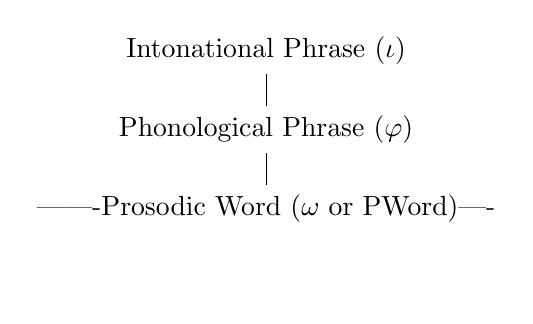
\begin{tikzpicture}[node distance = 1cm, auto]
				\node (6) [] {Intonational Phrase ($\iota$)}; 
				\node (5) [below of=6] {Phonological Phrase ($\varphi$)}; 
				\node (3) [below of=5] {-------Prosodic Word ($\omega$ or PWord)----}; 
				\node (2) [below of=3] { }; 
				
				\draw (6) -- (5);
				\draw (5) -- (3);
			\end{tikzpicture} 
			
			\ex ~\label{nlttPapertree hierarchy pstem redpaperhydbsbfsv}
			
			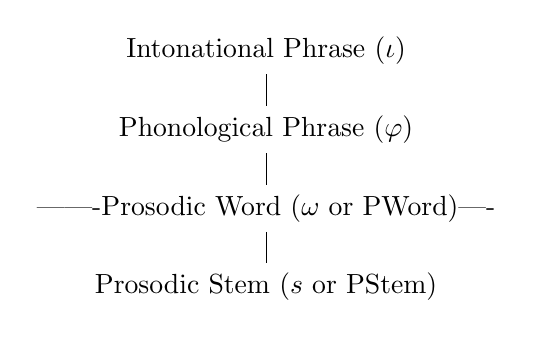
\begin{tikzpicture}[node distance = 1cm, auto]
				\node (6) [] {Intonational Phrase ($\iota$)}; 
				\node (5) [below of=6] {Phonological Phrase ($\varphi$)}; 
				\node (3) [below of=5] {-------Prosodic Word ($\omega$ or PWord)----}; 
				\node (2) [below of=3] {Prosodic Stem ($s$ or PStem)}; 
				
				\draw (6) -- (5);
				\draw (5) -- (3);
				\draw (3) -- (2);
			\end{tikzpicture}
		\end{xlist}
	\end{multicols}
	
\end{exe}

\begin{exe}
	\ex \label{nlttPapertree hierarchy table wesbdthewegashr}
	
	\begin{tabular}{ll}
		a. &b. \\
		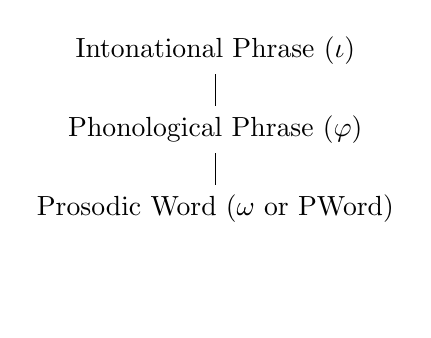
\begin{tikzpicture}[node distance = 1cm, auto]
			\node (6) [] {Intonational Phrase ($\iota$)}; 
			\node (5) [below of=6] {Phonological Phrase ($\varphi$)}; 
			\node (3) [below of=5] {Prosodic Word ($\omega$ or PWord)}; 
			\node (2) [below of=3] {\textcolor{white}{(}}; 
			
			\draw (6) -- (5);
			\draw (5) -- (3);
		\end{tikzpicture} 
		& 
		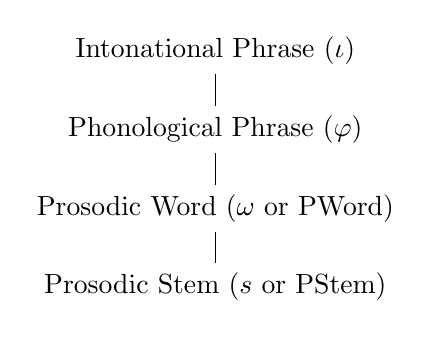
\begin{tikzpicture}[node distance = 1cm, auto]
			\node (6) [] {Intonational Phrase ($\iota$)}; 
			\node (5) [below of=6] {Phonological Phrase ($\varphi$)}; 
			\node (3) [below of=5] {Prosodic Word ($\omega$ or PWord)}; 
			\node (2) [below of=3] {Prosodic Stem ($s$ or PStem)}; 
			
			\draw (6) -- (5);
			\draw (5) -- (3);
			\draw (3) -- (2);
		\end{tikzpicture}
		
	\end{tabular}
	\begin{multicols}{2}
		
		\begin{xlist}
			\ex ~\label{nlttPapertree hierarchy traditional redpaperhydbsbfsv} 
			
			
			\ex ~\label{nlttPapertree hierarchy pstem redpaperhydbsbfsv}
			
		\end{xlist}
	\end{multicols}
	
\end{exe}


Just as syntactic phrases and morphological words are the sources of prosodic phrases and prosodic words, MStems are the source of PStems. The bulk of the evidence for the PStem comes from agglutinative languages and language families \citep{CzaykowskaHiggins-1997-MorphologicalPhonoConstituentSalish,Downing-2016-ProsodicLevelsChichewa}. The diagnostics used to detect PStems in other languages also show the PStem in Armenian. In Armenian, the overapplication of DHR straddles the boundary between the MStem and V-initial inflection. In other agglutinative languages, stem-level processes have been shown to be sensitive to the syllabification of MStems with V-initial suffixes or C-final prefixes. 
To illustrate, \citet{Aronoff-1988-HeadOperationsStrateRED} analyzes reduplication in KiHehe as targetting the morphological stem of the word (in italics). The reduplicant (underlined) is linearly found between inflectional prefixes and the stem (\ref{nlttPaperkihehe c redpapergbbdff}). The reduplicant generally copies only stem segments. But when the stem is V-initial, prefix-final consonants are copied because of syllabification (\ref{nlttPaperkihehe v redpapergbbdff}). 











\begin{exe}
	\ex 
	\begin{multicols}{2}
		\begin{xlist}
			\ex \makebox[3cm][l]{\textipa{ku-\textit{haata}}}`to ferment'\label{nlttPaperkihehe c redpapergbbdff}\\
			\makebox[3cm][l]{\textipa{ku-\underline{haata}$\sim${\textit{haata}}}}`to start fermenting'
			\ex \makebox[3cm][l]{\textipa{kw-\textit{iita}}}`to pour'\label{nlttPaperkihehe v redpapergbbdff}\\
			\makebox[3cm][l]{\textipa{\underline{kw-iita}$\sim${kw-\textit{iita}}}}`to start pouring'
		\end{xlist}
		
	\end{multicols}
\end{exe}

To explain prefix-copying in V-initial stems, \citet{Aronoff-1988-HeadOperationsStrateRED} analyzes reduplication as also targeting a prosodic head but does not formalize this concept. \citet{Downing-1998-ProsodicMisalignmentReduplication} reanalyzes KiHehe and formalizes the prosodic head as the PStem. It is mapped from the MStem, but it misaligns because of syllabification.

As a constituent, the PStem can be the target of reduplication, tonal processes, vowel harmony, minimality, and other sublexical processes \citep{Downing-1998-ProsodicMisalignmentOnsetlessNLLT,Downing-1999-ProsodicStem,Downing-1999-VerbalRed3BantuLanguages}. Further evidence for the PStem as a domain for phonological rules comes from cross-linguistic work on reduplication \citep{FitzpatrickCole-1994-ProsodicHierarchyReduplication,InkelasZoll2005-MorphoDouble,Shaw-2005-NonAdjacencyRed}, prefix-suffix asymmetries \citep{Hyman-2008-DirectionalAsymmetries}, minimality \citep{Downing-2005-MorphoCompelexityProsodicMinimality,Downing-2006-CanonicalForms}, strata \citep{Inkelas-1989-ProsodicLexicon,Inkelas-1993-DerivingCyclicity}, problems in bracket erasure \citep{Inkelas-2014-Interplay}, and bracketing paradoxes in compounds \citep{Han-1995-ProsodicStructureCompounds}. For a summary of the cross-linguistic evidence for the PStem, see \citet{Downing-2006-CanonicalForms,Downing-2016-ProsodicLevelsChichewa}, \citeauthor{DowningKadenge-2020-ReplacingPStemProsodicHierarchy} (to appear).

\subsubsection{The Prosodic Stem in Armenian}\label{nlttPapersection: reduction: destressed reduction EA: pstem: apply}
Applying the PStem to Armenian, I argue that MStems are mapped to non-recursive PStems while MWords are mapped to PWords. Before V-initial inflection, the PStem is misaligned from the MStem and expands. Before C-initial inflection, the PStem stays isomorphic with the MStem.


\begin{exe}
	\ex \textit{Different PStem structures in the two Armenian dialects.}\label{nlttPapertable: prosodic trees of EA WA} 
	
	\hspace*{-1cm}		\begin{tabular}{l|| l|l|l|l}
		\hline
		Type of structure&Base&Derivative&V-initial inflection&C-initial inflection\\\hline
		Morphology&
		\begin{tikzpicture}[scale = 0.8]
			
			\Tree [.MWord [.MStem \edge[roof];{{/\textipa{ɑmusin}/} -$\emptyset$} ] [.\textsc{nom} $\emptyset$ ] ] 
			
			
		\end{tikzpicture}
		&
		\begin{tikzpicture}[scale = 0.8]
			
			\Tree [.MWord [.MStem [.{MStem} \edge[roof];{{/\textipa{ɑmusin}/} -$\emptyset$} ] [.a /\textipa{-utjun}/ ] ] [ [.\textsc{nom} $\emptyset$ ] ] ] 
			
			
		\end{tikzpicture}
		&
		\begin{tikzpicture}[scale = 0.8]
			
			\Tree [.MWord [.MStem \edge[roof];{{/\textipa{ɑmusin}/} -$\emptyset$} ] [.{\ins} /\textipa{-ov}/ ] ] 
		\end{tikzpicture}
		&
		\begin{tikzpicture}[scale = 0.8]
			
			\Tree [.MWord [.MStem \edge[roof];{{/\textipa{ɑmusin}/} -$\emptyset$} ] [.{\pl} /\textipa{-ner}/ ] ] 
			
			
			
		\end{tikzpicture}
		\\\hline
		Prosody&
		\begin{tikzpicture}[scale = 0.75]
			\Tree [.PWord [.PStem \edge[roof];\textipa{ɑmus\'in} ] 					] 
			
			%	\Tree [.{Not Western Armenian} \edge[color=white];[.PWord [.PStem amusn-\'i ] ] 					]
			
		\end{tikzpicture}
		&
		\begin{tikzpicture}[scale = 0.75]
			\Tree [.PWord [.PStem \edge[roof];\textipa{ɑmusn-utj\'un} ] 					] 
			
			%	\Tree [.{Not Western Armenian} \edge[color=white];[.PWord [.PStem amusn-\'i ] ] 					]
			
		\end{tikzpicture}
		&
		\begin{tikzpicture}[scale = 0.75]
			
			\Tree [.PWord [.PStem \edge[roof];\textipa{ɑmus(i)n-\'ov} ] ] 				 
		\end{tikzpicture}
		&
		\begin{tikzpicture}[scale = 0.75]
			\Tree [.PWord [.PStem \edge[roof];\textipa{ɑmusin} ] [.$\sigma$ \textipa{-n\'er} ] 					] 
			
			%	\Tree [.{Not Western Armenian} \edge[color=white];[.PWord [.PStem amusn-\'i ] ] 					]
			
		\end{tikzpicture}
		\\\hline
		
		
	\end{tabular}
	
\end{exe} 



I argue that the PStem is indexed with its own cophonology. In EArm, the PStem triggers Stress Shift and Destressed High Vowel Reduction (DHR) but not Destressed Diphthong \textit{uj-}Reduction (DDR).\footnote{In order for the EArm PStem-level cophonology to trigger high vowel reduction but not diphthong reduction, we need the ranking: \textsc{*Reduce^2} $>>$ *\textit{\v{i},\v{u}} $>>$ {\textsc{ Id[f]} $>>$ \textsc{Max-V}} $>>$ *\textit{\v{uj}}. The faithfulness constraints \textsc{Id[f],Max-V} are outranked by *\textit{\v{i},{u}}. This triggers high vowel reduction. However, these faithfulness constraints outrank *\textit{\v{uj}}. This ranking blocks *\textit{\v{uj}} from triggering high diphthong reduction. The constraint \textsc{*Reduce^2} also dominates *\textit{\v{i},\v{u}}. This prevents \text{*\textit{\v{i},\v{u}}} from triggering diphthong reduction. \label{nlttPaperfootnote destressed diphtohng pstem}
} This is more than the stem-level cophonology, and less than the word-level cophonology. In WArm, the PStem cophonology is equivalent to the word-level stratum. It triggers stress shift but not reduction. 







\begin{exe}
	\ex \textit{Distribution of processes and domains across cophonologies}\\
	
	\begin{tabular}{l | llll}
		Morphological domain&Derivation&\multicolumn{2}{c}{V-initial Inflection}&Inflection\\
		Relevant constituent&MStems&\multicolumn{2}{c}{Misaligned PStems}&MWords\\
		Cophonology&Stem-level&\multicolumn{2}{c}{PStem-level}& Word-level\\
		% Domain&MStems&\mulExpanded PStem=MStem + V-Infl.&MWord\\
		\hline
		backslashbox[71mm]{Process}{Dialect} &Both&EArm&WArm&Both\\\cline{2-5}
		Destressed Diphthong \textit{uj} Reduction (DDR) &\ding{51} &\ding{55} &\ding{55} &\ding{55} \\
		Destressed High Vowel Reduction (DHR)&\ding{51} &\ding{51} &\ding{55} &\ding{55} \\
		Stress Shift &\ding{51} &\ding{51} &\ding{51} &\ding{51} \\
		
	\end{tabular}
\end{exe}


The stem-level and word-level strata are morphologically triggered by derivation and inflection. In contrast, the PStem-level cophonology is an intermediate cophonology: it applies after the stem-level and before the word-level when the right prosodic conditions are met. Specifically, it applies when V-initial inflection is added to an MStem and PStem misalignment: \textit{\textipa{//(a.mu.si.n)_s-ov// $\rightarrow$(a.mu.si.n-ov)_s}}. I stipulate that the PStem-cophonology \textit{only} occurs when we have PStem misalignment. I formalize the constraints needed (S\ref{nlttPapersection: reduction: destressed reduction EA: pstem: apply: constreaint}) to generate the PStem in uninflected (S\ref{nlttPapersection: reduction: destressed reduction EA: pstem: apply: der}) and inflected words (S\ref{nlttPapersection: reduction: destressed reduction EA: pstem: apply: infl}).

\subsubsubsection{Overview and constraint definitions}\label{nlttPapersection: reduction: destressed reduction EA: pstem: apply: constreaint} 

I use the following constraints adapted from \textsc{Match} theory \citep{Selkirk-2011-SyntaxPhonoInterface}. I have adapted them for mapping PStems \citep{Downing-1999-VerbalRed3BantuLanguages}, for mapping nested domains (\ref{nlttPaperconstraint: pstem wrapstem redpapertgdfsnd}; \citealt{Truckenbrodt-1999-RelationSyntaxPhonologyWRAP}), and for mapping non-isomorphic PStems (\ref{nlttPaperconstraint: pstem overmatch redpapertgdfsnd},\ref{nlttPaperconstraint: pstem undermatch redpapertgdfsnd}; \citealt{Guekguezian-2017-ProsodicRecursionCyclicityWord,Guekguezian-2017-TemplatesInteractionRecursionWordProsodic}). 



\begin{exe}
	\ex 
	\begin{xlist}
		\ex \textsc{MatchStem} $\sim$ \textsc{Match}: An MStem must correspond to a PStem\label{nlttPaperconstraint: pstem match redpapertgdfsnd}
		\ex \textsc{OverMatch} $\sim$ \textsc{Over}: A PStem does not contain a segment which isn't in its MStem (= overparse)\label{nlttPaperconstraint: pstem overmatch redpapertgdfsnd}
		\ex \textsc{UnderMatch} $\sim$ \textsc{Under}: A PStem does not lack a segment which isn't in its MStem (= underparse)\label{nlttPaperconstraint: pstem undermatch redpapertgdfsnd}
		\ex \textsc{AlignSyll} $\sim$ \textsc{Align}: A PStem must be aligned with syllable boundaries \label{nlttPaperconstraint: pstem alignsyll redpapertgdfsnd}
		\ex \textsc{NonRec}: PStems cannot be recursive\label{nlttPaperconstraint: pstem nonrec redpapertgdfsnd}
		\ex \textsc{WrapStem} or $\sim$ \textsc{Wrap}: An MStem must either a) correspond to a PStem, or b) be dominated by an MStem which corresponds to a PStem\label{nlttPaperconstraint: pstem wrapstem redpapertgdfsnd}
		
		
	\end{xlist}
\end{exe}

Contra \citet{Selkirk-2011-SyntaxPhonoInterface}, \citet{Elfner-2015-RecursionProsodicPhrasingIrish}, and \citet{Truckenbrodt-1999-RelationSyntaxPhonologyWRAP}, I define these constraints in terms of correspondence, not in terms of matching terminal nodes. I use the term `mapping' to mean the creation of PStems and of establishing a correspondence relationship between MStems and PStems \citep[cf. correspondence relations in ][]{MccarthyPrince-1995-Reduplication,itoMester-2019-matchSyntaxProsodyMaxDepProsodicEnclisisEnglish}. The constraint \textsc{MatchStem} requires that an MStem is mapped to a PStem, i.e., it is in correspondence with a PStem. The constraint does not require that a PStem contains all, only, or any of the segments of the MStem. The constraints \textsc{UnderMatch}, \textsc{OverMatch} handle what segments are contained in the PStem. \textsc{WrapStem} is a weaker version of \textsc{MatchStem} that allows an MStem's segments to be parsed into a higher MStem's PStem.%. A MStem is wrapped into a PStem by being in correspondence with the PStem, or by being dominated by a larger MStem which is in correspondence with the PStem. %If a candidate violates \textsc{WrapStem} then it also violates \textsc{MatchStem}; but a candidate can violate \textsc{MatchStem} without violating \textsc{WrapStem}. The constraint \textsc{MatchStem} will be shown to be inactive due to high-ranking \textsc{NonRec} and \textsc{WrapStem}. %ithat the MStem is in correspo It requires .% They are ranked differently in WArm and EArm, showing that the dialects vary in some but not all of their prosodic constraints The constraints \textsc{AlignSyll}, \textsc{NonRec}, and \textsc{WrapStem} are undominated and not violated on the surface.

\subsubsubsection{Mapping non-recursive PStems in roots and derivatives}\label{nlttPapersection: reduction: destressed reduction EA: pstem: apply: der}

In (\ref{nlttPaperderivation table: stratal prosody amusin amusnutjun}), I show the condensed cyclic derivation of the free-standing root \textit{\textipa{ɑmusi\'n}} and its derivative \textit{\textipa{ɑmusn-utj\'un}}. I use an explicit prosody step for syllabification and PStem mapping. Both uninflected MStems are parsed to a single non-recursive PStem. Without PStem misalignment, these words don't undergo the PStem-cophonology. MStems are marked with \{...\}\textsubscript{S} in the input, PStems with (...)\textsubscript{s} in the output. 

% \begin{exe}
	
	% \ex 
	% \begin{xlist}
		
		% \ex \makebox[3cm][l]{Base}\makebox[3cm][l]{\textipa{ɑmus\'in}}\makebox[3cm][l]{`husband'}\label{nlttPaperexample: warm earm reduce high list repeat: base} 
		% \ex \makebox[3cm][l]{Der. Suffix}\makebox[3cm][l]{\textipa{ɑmusn-utj\'un}}\makebox[3cm][l]{`marriage'}\label{nlttPaperexample: warm earm reduce high list repeat: der} 
		% %\ex \makebox[3cm][l]{Compound}\makebox[3cm][l]{\textipa{s\'er}}\makebox[3cm][l]{`love'}\label{nlttPaperexample: warm earm reduce high list repeat: compound}\\
		% %\makebox[3cm][l]{}\makebox[3cm][l]{\textipa{ɑmusn-a-s\'er}}\makebox[3cm][l]{`loving one's husband'} 
		% \ex \makebox[3cm][l]{V-initial Infl.}\makebox[3cm][l]{\textipa{ɑmusn-\'ov}}\makebox[4cm][l]{`husband-{\ins}'}EArm\label{nlttPaperexample: warm earm reduce high list repeat: V inf ea} 
		% \ex \makebox[3cm][l]{}\makebox[3cm][l]{\textipa{ɑmusin-\'ov}}\makebox[4cm][l]{`husband-{\ins}'}WArm\label{nlttPaperexample: warm earm reduce high list repeat: V inf wa} 
		% \ex \makebox[3cm][l]{C-initial Infl.}\makebox[3cm][l]{\textipa{ɑmusin-n\'er}}\makebox[4cm][l]{`husband-{\pl}'}EArm, WArm\label{nlttPaperexample: warm earm reduce high list repeat: C inf both}
		% \end{xlist}\label{nlttPaperexample: warm earm reduce high list repeat}
	
	
	% \end{exe}

















\begin{exe}
	\ex \textit{Stratal and prosodic derivation of the root} \textipa{ɑmusin} \textit{and its derivative} \textipa{ɑmusn-utjun} \label{nlttPaperderivation table: stratal prosody amusin amusnutjun}\\
	
	\begin{tabular}{||llll l|| ll||}
		\hline
		
		% &&&
		% \begin{tikzpicture}[scale = 0.8]
			
			% 		\Tree [.MW_{\textsc{nom}} [.MS_{\textit{n}} [.$\sqrt{}$ /\textipa{ɑmusin}/ ] [.n -$\emptyset$ ] ] [ [.\textsc{nom} -$\emptyset$ ] ] ]
			
			% 		\end{tikzpicture} 
		% &
		% \begin{tikzpicture}[scale = 0.8]
			
			% 		\Tree [.MW_{nom} [.MS_{\textit{n}} [. MS_{\textit{n}} [.$\sqrt{}$ /\textipa{ɑmusin}/ ] [.n -$\emptyset$ ] ] ] [ [ [.n /\textipa{-utjun}/ ] ] ] ]
			
			% 		\end{tikzpicture} 
		
		% \\
		Input & &&& \textipa{/amusin -$\emptyset$_{S} /} & &\textipa{/amusin -$\emptyset$_{S1} -utjun_{S2}/} \\\hline\hline
		\textit{Cycle 1}& \textsc{Morph}& &Spell-out & \textipa{/amusin -$\emptyset$_{S} /} &\textit{Cycle 2} & \textipa{(a.mu.s\'in)_{s1} - /-utjun_{S2}}/ \\
		& \textsc{Prosody} &&Syllabify & \textipa{ɑ.mu.s\'in} & & \textipa{(a.mu.si.n)_{s1}-u.tjun} \\ 
		& &&Map PStem & \textipa{(a.mu.s\'in)_{s}} &&
		\textipa{(a.mu.si.n-u.tjun)_{s2}} \\
		& \textsc{Phono}& \textit{SLevel} &Stress & \textipa{(a.mu.s\'in)_{s}}& &\textipa{(a.mu.s\v{i}.n-u.tj\'un)_{s2}} \\
		&&&DHR && &\textipa{(a.mus.n-utj\'un)_s} 
		\\
		% && DHR & & \\
		% \hline
		% \\
		
		
		% \\
		% \\
		% \\
		% \hline
		% Cycle 3&\textsc{Morph}& Spell-out &\textipa{(amus\'in)_s /-$\emptyset$_W/} &\textipa{(amusn-utj\'un)_s /-$\emptyset$_W/} \\
		% & \textsc{Prosody} & Map PWord & \textipa{((amus\'in)_s)_w}& \textipa{((amusn-utj\'un)_s)_w} \\
		% & \textsc{Phono} & \textit{WLevel} & & \\
		% & & Stress & \textipa{((amus\'in)_s)_w}& \textipa{((amusn-utj\'un)_s)_w} \\
		
		\hline\hline
		Output& &&&\textipa{ɑmus\'in} && \textipa{ɑmusn-utj\'un} \\
		\hline 
	\end{tabular}
	
\end{exe}























In both dialects, a free-standing root forms an MStem that is mapped to an isomorphic PStem: \textit{\textipa{(amusin)_{s}}} (\ref{nlttPaperot tableau: base amusin}d). This is mandated by the parsing constraints \textsc{MatchStem} and \textsc{WrapStem} which are violated by the unparsed candidate (\ref{nlttPaperot tableau: base amusin}a). Constraint \textsc{UnderMatch} blocks candidates where no MStem segments are parsed (\ref{nlttPaperot tableau: base amusin}b), or only some are (\ref{nlttPaperot tableau: base amusin}c). Losing candidates (b,c) satisfy \textsc{MatchStem} because the MStem is in correspondence with a PStem, regardless of what the PStem contains. 






\begin{exe}
	\ex ~\\
	
	\vspace{-1cm}\label{nlttPaperot tableau: base amusin}\renewcommand*\arraystretch{1.2}
	\scalebox{1}[1]{\begin{tabular}[t]{|rrl||c:c:c:c:c:c|} \hline
			\multicolumn{3}{|c||}{\textipa{\{amusin\}_{S}}} & \textsc{Align} & \textsc{NonRec} & \textsc{Wrap} & \textsc{Match} & \textsc{Under} & \textsc{Over} \\[0.5ex]
			% \multicolumn{3}{|c||}{}& \textsc{Syll} & \textsc{} & \textsc{Stem} & \textsc{Stem} & \textsc{Match} & \textsc{Match} \\[0.5ex]
			
			% \multicolumn{3}{|c||}{} & \textsc{Syll} & \textsc{} & \textsc{Stem} & \textsc{Stem} & \textsc{Match} & \textsc{Match} \\[0.5ex]
			\hline
			\hline a. & & \textipa{ɑmusin} & & & $\ast$ & $\ast$ & & \\
			\hline b. & & \textipa{()_{s}amusin} & & & & & $\ast\ast\ast\ast\ast\ast$ & \\
			\hline c. & & \textipa{(amu)_{s}sin} & & & & & $\ast\ast\ast$ & \\
			\hline d. & \ding{43} & \textipa{(amusin)_{s}} & & & & & & \\
			\hline \end{tabular}} \renewcommand*\arraystretch{1} 
	
\end{exe}







In derived words like \textit{\textipa{ɑmusn-utjun}}, the two MStems are mapped to a single PStem: \textit{\textipa{(a.mu.si.n-utjun)_{s2}}} (\ref{nlttPaperot tableau: der amsuinutjun}k). The different numerical subscripts \textsubscript{1,2} 
mark the correspondence of different stems. The inner MStem \textit{S1} does not correspond to a PStem (= violates \textsc{MatchStem}) but it is dominated by an MStem which does have a PStem (= satisfies \textsc{WrapStem}). The required ranking is that \textsc{AlignSyll, NonRec, WrapStem} outrank \textsc{MatchStem}. I remove stress marks to reduce clutter.












\begin{exe}
	\ex ~\\
	
	\vspace{-1cm} \label{nlttPaperot tableau: der amsuinutjun} \resizebox{1\textwidth}{!}{%
		\renewcommand*\arraystretch{1.2}
		\scalebox{1}[1]{\begin{tabular}[t]{|l|rrl||c:c:c|c:c:c|} \hline
				&\multicolumn{3}{|c||}{\textipa{\{\{amusin\}_{S1}-utjun\}_{S2}}} & \textsc{Align} & \textsc{NonRec} & \textsc{Wrap} & \textsc{Match} & \textsc{Under} & \textsc{Over} \\[0.5ex]
				% &\multicolumn{3}{|c||}{}& \textsc{Syll} & \textsc{} & \textsc{Stem} & \textsc{Stem} & \textsc{Match} & \textsc{Match} \\[0.5ex]
				\hline \hline 
				\textit{Recursive }& a. & & \textipa{((amusi.n-u)_{s1}tjun)_{s2}} & & $\ast$! & & \cellcolor{lightgray} & \cellcolor{lightgray} & \cellcolor{lightgray}$\ast$ \\\cline{5-10}
				\textit{Candidates}& b. & & \textipa{((amusi.n)_{s1}-utjun)_{s2}} & $\ast$! & $\ast$! & & \cellcolor{lightgray} & \cellcolor{lightgray} & \cellcolor{lightgray} \\ \cline{5-10}
				& c. & & \textipa{((amusi)_{s1}n-utjun)_{s2}} & & $\ast$! & & \cellcolor{lightgray} & \cellcolor{lightgray}$\ast$ & \cellcolor{lightgray} \\
				
				\hline
				\textit{Unwrapped}
				& d. & & \textipa{(amusin-u)_{s1}tjun} & & & $\ast$! & \cellcolor{lightgray}$\ast$ & \cellcolor{lightgray} & \cellcolor{lightgray}$\ast$ \\\cline{5-10}
				\textit{Candidates}
				&e. & & \textipa{(amusi.n)_{s1}utjun} & $\ast$! & & $\ast$! & \cellcolor{lightgray}$\ast$ & \cellcolor{lightgray} & \cellcolor{lightgray} \\\cline{5-10}
				&f. & & \textipa{(amusi.)_{s1}n-utjun} & & & $\ast$! & \cellcolor{lightgray}$\ast$ & \cellcolor{lightgray}$\ast$ & \cellcolor{lightgray} \\
				\hline 
				\textit{Underparsed}
				&g. & & \textipa{(amusin-u)_{s2}tjun} & & & & $\ast$ & $\ast$!$\ast \ast \ast$ & \\
				\cline{5-10}
				\textit{Candidates}&h. & & \textipa{(amusi.n)_{s2}utjun} & $\ast$! & & & \cellcolor{lightgray}$\ast$ & \cellcolor{lightgray}$\ast \ast \ast \ast \ast$ & \cellcolor{lightgray} \\ \cline{5-10}
				&i. & & \textipa{(amusi.)_{s2}n-utjun} & & & & $\ast$ & $\ast$!$\ast \ast \ast \ast \ast$ & \\
				\hline \textit{Overparsed C.}& j. & & \textipa{(amusin-utjun)_{s1}} & & & $\ast$! & \cellcolor{lightgray}$\ast$ & \cellcolor{lightgray} & \cellcolor{lightgray}$\ast \ast \ast \ast \ast$ \\
				\hline &k. & \ding{43} & \textipa{(amusin-utjun)_{s2}} & & & & $\ast$ & & \\
				\hline \end{tabular}} \renewcommand*\arraystretch{1}
	}
\end{exe}

The constraints \textsc{AlignSyll, NonRec, WrapStem} are inviolable. High-ranking \textsc{AlignSyll} blocks candidates (\ref{nlttPaperot tableau: der amsuinutjun}b,e,h) where the PStem is not aligned with syllable boundaries: \textit{\textipa{(amusi.n)_{s1}utjun}} (b). High-ranking \textsc{NonRec} blocks candidates with recursive structure (a,b,c). High-ranking \textsc{WrapStem} blocks candidates (d,e,f) where the larger MStem \textit{S2} is not mapped to any PStem: \textit{\textipa{(amusin)_{s1}-utjun}} (e). Candidates (g,h,i) violate \textsc{UnderMatch} because MStem \textit{S2} is mapped to a small PStem \textit{s2}: \textit{\textipa{(amusin)_{s2}-utjun}} (h). The last losing candidate has MStem \textit{S1} map to a large PStem \textit{s1}: \textit{\textipa{(amusin-ujtun)_{s1}}}. Even though all the segments of MStem \textit{S2} are parsed inside a PStem $s1$, the candidate violates \textsc{WrapStem} because the larger MStem \textit{S2} is not in correspondence with any PStem.\footnote{I omit one logically possible candidate: \textit{\textipa{(amusinu-utjun)_{s1,2}}}. This candidate has a single large PStem. This PStem is in correspondence with both MStems. It only violates \textsc{OverMatch} because the PStem has 5 segments \textit{-utjun} which aren't in MStem \textit{S1}. It does not violate \textsc{MatchStem} or \textsc{WrapStem} because the MStems do have a correspondent PStem; these correspondents just happen to be the same PStem. I assume this candidate is not generated because a PStem cannot have multiple correspondents. 
} 


\subsubsubsection{Mapping misaligned PStems in inflection}\label{nlttPapersection: reduction: destressed reduction EA: pstem: apply: infl}

Before inflection, the shape of the PStem varies depending on the shape of the inflectional suffix. Briefly, V-initial inflection triggers resyllabification and PStem expansion. I \textit{stipulate} that PStem misalignment triggers the PStem-cophonology. This cophonology includes DHR in EArm. I illustrate below for the different inflected items with V-initial inflection: \textit{\textipa{ɑmusn-\'ov}} (EArm), \textit{\textipa{ɑmusin-\'ov}} (WArm), and C-initial inflection: \textit{\textipa{ɑmusin-n\'er}}. %The variation in the shape of the PStem is due to a constraint \textsc{AlignSyll} that requires PStems to align with syllable boundaries. % Table (\ref{nlttPaperderivation table: strata prosody amusinov amusnov amusinner}) illustrates this. 

















\begin{exe}
	\ex \textit{Stratal and prosodic derivation of} \textipa{ɑmusn-ov} (EArm), \textipa{ɑmusin-ov} (WArm), \textit{and} \textipa{ɑmusin-ner} (both)\label{nlttPaperderivation table: strata prosody amusinov amusnov amusinner}\\
	
	\hspace*{-1.25cm}\resizebox{1.05\textwidth}{!}{%\hspace*{-1.2cm}
		\begin{tabular}{||lll l| lll||}
			\hline
			&&&&EArm & WArm & EArm \&WArm\\
			
			% &&&
			% \begin{tikzpicture}[scale = 0.8]
				
				% 		\Tree [.MW_{{\ins}} [.MS_{\textsc{n}} [.$\sqrt{}$ /\textipa{ɑmusin}/ ] [.\textit{n} -$\emptyset$ ] ] [ [.{\ins} \textipa{/-ov/} ] ] ] 
				
				% 		\end{tikzpicture} 
			% &
			% \begin{tikzpicture}[scale = 0.8]
				
				% 		\Tree [.MW_{{\ins}} [.MS_{\textsc{n}} [.$\sqrt{}$ /\textipa{ɑmusin}/ ] [.\textit{n} -$\emptyset$ ] ] [ [.{\ins} \textipa{/-ov/} ] ] ] 
				
				% 		\end{tikzpicture} 
			% &
			% \begin{tikzpicture}[scale = 0.8]
				
				% 		\Tree [.MW_{{\pl}} [.MS_{\textsc{n}} [.$\sqrt{}$ /\textipa{ɑmusin}/ ] [.\textit{n} -$\emptyset$ ] ] [ [.{\pl} \textipa{/-ner/} ] ] ] 
				
				% 		\end{tikzpicture} 
			
			% \\
			Input & && &\textipa{/amusin -$\emptyset$_S -ov_W/} & \textipa{/amusin -$\emptyset$_S -ov_W/} & \textipa{/amusin -$\emptyset$_S -ner_W/} \\\hline\hline
			Cycle 1 & & & & \textipa{(a.mu.s\'in)_s} & \textipa{(a.mu.s\'in)_s} & \textipa{(a.mu.s\'in)_s} \\
			\hline\hline
			Cycle 2 &\textsc{Morph}&& Spell-out & \textipa{(a.mu.s\'in)_s - /-ov_W}/ & \textipa{(a.mu.s\'in)_s - /-ov_W}/ & \textipa{(a.mu.s\'in)_s - /-ner_W}/ \\
			%Cycle 2a 
			& \textsc{Prosody} &&Syllabify &\textipa{(a.mu.s\'i.n)_s-ov}&\textipa{(a.mu.s\'i.n)_s-ov}&\textipa{(a.mu.s\'in)_s-ner} \\
			% Cycle 2b
			& && Readjust PStem &\textipa{(a.mu.s\'i.n-ov)_s}&\textipa{(a.mu.s\'i.n-ov)_s}& \\
			% & & Map PWord &\textipa{((a.mu.si.n-ov)_s)_w}&\textipa{((a.mu.sin-ov)_s)_w}&{\textipa{((amusin)_s-ner)_w}} \\\hline
			% Cycle 2c 
			& \textsc{Phono}& \textit{PStem-level} & Stress &\textipa{(a.mu.s\v{i}.n-\'ov)_s}&\textipa{(a.mu.s\v{i}.n-\'ov)_s}&\cellcolor{lightgray} \\
			&&& DHR (EArm) & \textipa{(a.mus.n-\'ov)_s}&\cellcolor{lightgray}&\cellcolor{lightgray} \\
			% \hline
			% Cycle 2d & \textsc{Phono}& \textit{PStem-level} (WArm) &\cellcolor{lightgray} &&\cellcolor{lightgray} \\
			% && Stress &\cellcolor{lightgray}&\textipa{((a.mu.s\v{i}.n-\'ov)_s)_w}& \cellcolor{lightgray}\\
			% \hline
			% Cycle 2d 
			& \textsc{Phono} & \textit{WLevel}& Stress&\textipa{(a.mu.sn-\'ov)_s}&\textipa{((a.mu.sin-\'ov)_s}&\textipa{(a.mu.sin)_s-n\'er)}\\\hline\hline
			Output&&&& \textipa{ɑmusn-\'ov}&\textipa{ɑmusin-\'ov}&\textipa{ɑmusin-n\'er} \\
			\hline 
		\end{tabular}
	}
\end{exe}




Given the base \textit{\textipa{(a.mu.sin)_s}}, inflection is spelled out and syllabified in Cycle 2. 
Before C-initial inflection, the PStem stays isomorphic with the MStem and with syllable boundaries. C-initial inflection is PStem-external: \textit{\textipa{(a.mu.sin)_s-ner}}. Before V-initial inflection, the PStem becomes misaligned from syllable boundaries: \textit{\textipa{*(a.mu.si.n)_s-ov}}. To repair this, the PStem is readjusted by incorporating the V-initial inflectional suffix: \textit{\textipa{(a.mu.si.n-ov)_s}}. The PStem cophonology is then triggered for the misaligned PStems. EArm's PStem triggers stress and DHR \textit{\textipa{ɑmusn-\'ov}}, WArm's PStem only triggers stress \textit{\textipa{ɑmusin-\'ov}}. The MWord is mapped to a PWord, and the word-level phonology applies.% reduction in. For the C-initial suffix \textit{\textipa{(amusin)_s-ner}}, the PStem is not misaligned so the PStem-level cophonology does not apply. The PStem-level cophonology only applies for V-initial inflection: \textit{\textipa{(amusin-ov)_s}}. High vowel reduction is in the PStem-level cophonology of EArm but not of WArm. In EArm in Cycle 2c, the PStem-level cophonology applies with DHR: \textit{\textipa{(amusn-ov})_s}. But in WArm in Cycle 2d, the PStem-level cophonology applies without DHR: \textit{\textipa{(amusin-\'ov)_s}}. The PStem-level cophonology in WArm is thus the same as the word-level cophonology. The word-level cycle then applies for all inflected words. These various changes in PStem shape are formalized in the appendix by ranking \textsc{AlignSyll} with various \textsc{Match} constraints. 








% In Table (\ref{nlttPapertable: prosodic trees of EA WA}), I summarize the morphological and prosodic structure for the different items in (\ref{nlttPaperexample: warm earm reduce high list repeat}). For ease of contrast, the non-terminal nodes are labelled as MWords, PWords, MStems, and PStems. I show covert inflection for the root and derivative.



I formalize the prosody step in Cycle 2 where the PStem is potentially readjusted before inflection. Before C-initial inflection in \textit{amusin-ner}, the PStem is isomorphic with the MStem and syllable boundaries because it violates no parsing constraints: \textit{\textipa{(a.mu.sin)_s-ner}} (\ref{nlttPaperot tableau: c initiai inf}). The losing candidates are harmonically bounded by the winner.



\begin{exe}
	\ex ~\\
	
	\vspace{-1cm}\label{nlttPaperot tableau: c initiai inf} \renewcommand*\arraystretch{1.2}
	\scalebox{1}[1]{\begin{tabular}[t]{|rrl||c:c:c|c:c:c|} \hline
			\multicolumn{3}{|c||}{\textipa{\{amusin\}_{S}-ner}} & \textsc{Align} & \textsc{NonRec} & \textsc{Wrap} & \textsc{Match} & \textsc{Under} & \textsc{Over} \\[0.5ex]
			% \multicolumn{3}{|c||}{}& \textsc{Syll} & \textsc{} & \textsc{Stem} & \textsc{Stem} & \textsc{Match} & \textsc{Match} \\[0.5ex]
			\hline \hline a. & \ding{43} & \textipa{(amusin)_{s}-ner} & & & & & & \\
			\hline b. & & \textipa{(amusin-ner)_{s}} & & & & & & $\ast\ast\ast$ \\
			\hline c. & & \textipa{ɑmusin-ner} & & & $\ast$! & \cellcolor{lightgray}$\ast$ & \cellcolor{lightgray} & \cellcolor{lightgray} \\
			\hline \end{tabular}} \renewcommand*\arraystretch{1} 
	
\end{exe}

% So far, there is no ranking among the constraints. But before V-initial inflection, mismatches are created and we see the need for constraint ranking: high-ranked \textsc{AlignSyll, WrapStem}. Crucially, the dialects will have different rankings of \textsc{UnderMatch} and \textsc{OverMatch} \citep[cf.][]{Anttila-2002-MorpholConditionedPhonoAlternation}. 

In both dialects, misalignment or non-isomorphism occurs in V-initial inflection due to syllabification (\ref{nlttPaperot tableau: v inf}). The losing faithful candidate \textit{\textipa{(a.mu.si.n)_s-ov}} violates the undominated constraint \textsc{AlignSyll}. To repair this, the PStem can be either contracted \textit{\textipa{(a.mu.si)_sn-ov}} (= violate \textsc{UnderMatch}) or expanded \textit{\textipa{(a.mu.si.n-ov)_s}} (= violate \textsc{OverMatch}). I argue it expands in both dialects. This means {\textsc{OverMatch}} outranks \textsc{UnderMatch}. Both constraints are dominated by \textsc{AlignSyll}. Regardless of misalignment, a PStem must be formed because \textsc{WrapStem} is undominated (cf. candidate d).

\begin{exe}
	% \ex
	% \begin{xlist}
		\ex ~\\
		
		\vspace{-1cm}\label{nlttPaperot tableau: v inf WA}\label{nlttPaperot tableau: v inf} \renewcommand*\arraystretch{1.2}
		\scalebox{1}[1]{\begin{tabular}[t]{|rrl||c:c|c|c|} \hline
				\multicolumn{3}{|c||}{\textipa{\{amusin\}_{S}-ov}} & \textsc{Wrap} &\textsc{Align} & \textsc{Under} & \textsc{Over} \\[0.5ex]
				\hline \hline a. & & \textipa{(amusi.n)_{s}-ov} && $\ast$! & \cellcolor{lightgray} & \cellcolor{lightgray} \\
				\hline b. & & \textipa{(amusi)_{s}n-ov} & & & $\ast$! & \cellcolor{lightgray} \\
				\hline c. & \ding{43} & \textipa{(amusin-ov)_{s}} & & & & \cellcolor{lightgray}$\ast\ast$ \\
				\hline d. & & \textipa{ɑmusin-ov} & $\ast!$ & & \cellcolor{lightgray} & \cellcolor{lightgray} \\
				\hline \end{tabular}} \renewcommand*\arraystretch{1} 
		
		
		
		
		% \ex \textit{Mapping PStems in }/\textipa{ɑmusin-ov}/ [\textipa{ɑmusn-ov]} \textit{with V-initial inflection in Eastern Armenian}\label{nlttPaperot tableau: v inf EA}
		
		% \renewcommand*\arraystretch{1.2}
		% \scalebox{1}[1]{\begin{tabular}[t]{|rrl||c:c|c|c|} \hline
				% \multicolumn{3}{|c||}{\textipa{{amusin}_S-ov}} & \textsc{Wrap} &\textsc{AlignSyll} & \textsc{OverMatch} & \textsc{UnderMatch} \\[0.5ex]
				% \hline \hline a. & & \textipa{(amusi.n)_s-ov} && $\ast$! & \cellcolor{lightgray} & \cellcolor{lightgray} \\
				% \hline b. &\ding{43} & \textipa{(amusi)_sn-ov} & & & & \cellcolor{lightgray}$\ast$ \\
				% \hline c. & & \textipa{(amusin-ov)_{s}} & & & $\ast!\ast$& \cellcolor{lightgray} \\
				% \hline d. & & \textipa{ɑmusin-ov} & $\ast!$ & & \cellcolor{lightgray} & \cellcolor{lightgray} \\
				% \hline \end{tabular}} \renewcommand*\arraystretch{1} 
		
		% \end{xlist}
	
\end{exe}





% In Table (\ref{nlttPapertable: prosodic trees of EA WA}), I summarize the morphological and prosodic structure for the different items in (\ref{nlttPaperexample: warm earm reduce high list repeat}). For ease of contrast, the non-terminal nodes are labelled as MWords, PWords, MStems, and PStems. I show covert inflection for the root and derivative.




\section{old:dissPre-inflectional DHR in  the Prosodic Stem}\label{disssection: reduction: destressed reduction EA: pstem}

In modern Armenian DHR, the relevant morphological constituent is the MStem and the relevant cophonology is the stem-level cophonology.   In this section,  I argue that the relevant prosodic constituent \textit{X} is the Prosodic Stem or PStem \citep{Downing-1999-ProsodicStem}. I first summarize the  cross-linguistic evidence for the PStem, and show how the EArm data match that of other languages which have PStems. 

\subsubsection{The role of Prosodic Stems}\label{disssection: reduction: destressed reduction EA: pstem: role}

The traditional prosodic hierarchy assumes only three levels of morphosyntactically derived constituents: the prosodic word, the prosodic phrase, and the intonational phrase (\ref{disstree hierarchy traditional redchapterhydbsbfsv}).  However, there is  cross-linguistic work on morphologically complex languages  which  argues for a more enriched hierarchy that includes at least one constituent below the PWord: the Prosodic Stem (\ref{disstree hierarchy pstem redchapterhydbsbfsv}).\footnote{The Prosodic Root (PRoot) has also been posited as a constituent mapped from morphological roots. The evidence for the PRoots, however, is less than for PStems. } 



\begin{exe}
	\ex 
	\begin{multicols}{2}
		
		\begin{xlist}
			\ex ~\label{disstree hierarchy traditional redchapterhydbsbfsv} 
			
			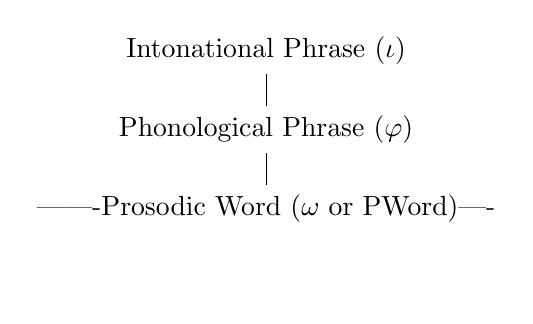
\begin{tikzpicture}[node distance = 1cm, auto]
				\node (6) [] {Intonational Phrase ($\iota$)}; 
				\node (5) [below of=6] {Phonological Phrase ($\varphi$)}; 
				\node (3) [below of=5] {-------Prosodic Word ($\omega$ or PWord)----}; 
				\node (2) [below of=3] { }; 
				
				\draw (6) -- (5);
				\draw (5) -- (3);
			\end{tikzpicture}  
			
			\ex ~\label{disstree hierarchy pstem redchapterhydbsbfsv}
			
			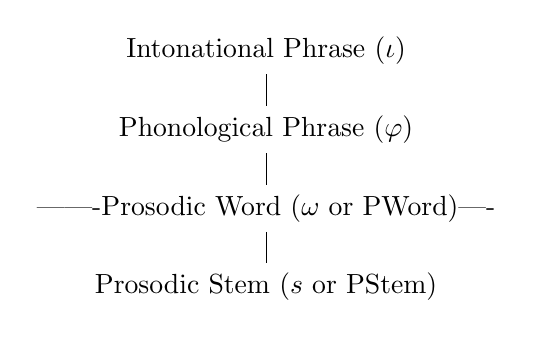
\begin{tikzpicture}[node distance = 1cm, auto]
				\node (6) [] {Intonational Phrase ($\iota$)}; 
				\node (5) [below of=6] {Phonological Phrase ($\varphi$)}; 
				\node (3) [below of=5] {-------Prosodic Word ($\omega$ or PWord)----}; 
				\node (2) [below of=3] {Prosodic Stem ($s$ or PStem)}; 
				
				\draw (6) -- (5);
				\draw (5) -- (3);
				\draw (3) -- (2);
			\end{tikzpicture}
		\end{xlist}
	\end{multicols}
	
\end{exe}



Just as syntactic phrases and morphological words are the sources of prosodic phrases and prosodic words, MStems are the source of   PStems.  The bulk of the evidence for the PStem comes from agglutinative languages and language families \citep{CzaykowskaHiggins-1997-MorphologicalPhonoConstituentSalish,Downing-2016-ProsodicLevelsChichewa}.  The diagnostics used to detect PStems in other languages  also show  the PStem in Armenian. In Armenian, the  overapplication of DHR straddles the boundary between the MStem and V-initial inflection. In other agglutinative languages, stem-level processes have been shown to be sensitive to the syllabification of MStems with V-initial suffixes or C-final prefixes. 
To illustrate,  \citet{Aronoff-1988-HeadOperationsStrateRED} analyzes   reduplication in KiHehe   as targetting the morphological stem of the word (in italics).  The reduplicant   (underlined) is linearly found between inflectional prefixes and the stem (\ref{disskihehe c redchaptergbbdff}).   The reduplicant generally copies only stem segments. But    when the stem is V-initial, prefix-final consonants are copied  because of syllabification (\ref{disskihehe v redchaptergbbdff}).  





\begin{exe}
	\ex 
	\begin{multicols}{2}
		\begin{xlist}
			\ex \makebox[3cm][l]{\textipa{ku-\textit{haata}}}`to ferment'\label{disskihehe c redchaptergbbdff}\\
			\makebox[3cm][l]{\textipa{ku-\underline{haata}$\sim${\textit{haata}}}}`to start fermenting'
			\ex \makebox[3cm][l]{\textipa{kw-\textit{iita}}}`to pour'\label{disskihehe v redchaptergbbdff}\\
			\makebox[3cm][l]{\textipa{\underline{kw-iita}$\sim${kw-\textit{iita}}}}`to start pouring'
		\end{xlist}
		
	\end{multicols}
\end{exe}

To explain  prefix-copying   in V-initial stems, \citet{Aronoff-1988-HeadOperationsStrateRED} analyzes reduplication as also targeting a prosodic head but does not formalize this concept.  \citet{Downing-1998-ProsodicMisalignmentReduplication} reanalyzes KiHehe   and formalizes the prosodic head as the PStem. It is mapped from the MStem, but it misaligns because of syllabification.

As a constituent, the PStem can be the target of reduplication, tonal processes, vowel harmony, minimality,  and other sublexical processes \citep{Downing-1998-ProsodicMisalignmentOnsetlessNLLT,Downing-1999-ProsodicStem,Downing-1999-VerbalRed3BantuLanguages}.   Further evidence for the PStem as a domain for phonological rules comes from cross-linguistic work on reduplication \citep{FitzpatrickCole-1994-ProsodicHierarchyReduplication,InkelasZoll2005-MorphoDouble,Shaw-2005-NonAdjacencyRed}, prefix-suffix asymmetries \citep{Hyman-2008-DirectionalAsymmetries}, minimality \citep{Downing-2005-MorphoCompelexityProsodicMinimality,Downing-2006-CanonicalForms}, strata \citep{Inkelas-1989-ProsodicLexicon,Inkelas-1993-DerivingCyclicity}, problems in bracket erasure \citep{Inkelas-2014-Interplay}, and   bracketing paradoxes in compounds \citep{Han-1995-ProsodicStructureCompounds}. For a summary of the cross-linguistic evidence for the PStem, see \citet{Downing-2006-CanonicalForms,Downing-2016-ProsodicLevelsChichewa},  \citeauthor{DowningKadenge-2020-ReplacingPStemProsodicHierarchy} (to appear).

\subsubsection{The Prosodic Stem in Armenian}\label{disssection: reduction: destressed reduction EA: pstem: apply}
Applying the PStem to Armenian, I argue that MStems are mapped to non-recursive PStems while MWords are mapped to PWords. Before V-initial inflection, the PStem is misaligned from the MStem and expands. Before C-initial inflection, the PStem stays isomorphic with the MStem.


\begin{exe}
	\ex  \textit{Different PStem structures   in the two Armenian dialects.}\label{disstable: prosodic trees of EA WA} 
	
	\hspace*{-1cm}		\begin{tabular}{l|| l|l|l|l}
		\hline
		Type of structure&Base&Derivative&V-initial inflection&C-initial inflection\\\hline
		Morphology&
		\begin{tikzpicture}[scale = 0.8]
			
			\Tree [.MWord [.MStem \edge[roof];{{/\textipa{ɑmusin}/}  -$\emptyset$} ]    [.\textsc{nom} $\emptyset$ ] ]  
			
			
		\end{tikzpicture}
		&
		\begin{tikzpicture}[scale = 0.8]
			
			\Tree [.MWord [.MStem [.{MStem} \edge[roof];{{/\textipa{ɑmusin}/}  -$\emptyset$} ]   [.a /\textipa{-utjun}/ ] ]   [ [.\textsc{nom} $\emptyset$ ] ] ]  
			
			
		\end{tikzpicture}
		&
		\begin{tikzpicture}[scale = 0.8]
			
			\Tree [.MWord [.MStem \edge[roof];{{/\textipa{ɑmusin}/}  -$\emptyset$} ]   [.\textsc{inst} /\textipa{-ov}/ ] ]  
		\end{tikzpicture}
		&
		\begin{tikzpicture}[scale = 0.8]
			
			\Tree [.MWord [.MStem \edge[roof];{{/\textipa{ɑmusin}/}  -$\emptyset$} ]   [.\textsc{pl} /\textipa{-ner}/ ] ]  
			
			
			
		\end{tikzpicture}
		\\\hline
		Prosody&
		\begin{tikzpicture}[scale = 0.75]
			\Tree [.PWord [.PStem \edge[roof];\textipa{ɑmus\'in} ] 					] 
			
			%	\Tree [.{Not Western Armenian} \edge[color=white];[.PWord [.PStem amusn-\'i ] ] 					]
			
		\end{tikzpicture}
		&
		\begin{tikzpicture}[scale = 0.75]
			\Tree [.PWord [.PStem \edge[roof];\textipa{ɑmusn-utj\'un} ] 					] 
			
			%	\Tree [.{Not Western Armenian} \edge[color=white];[.PWord [.PStem amusn-\'i ] ] 					]
			
		\end{tikzpicture}
		&
		\begin{tikzpicture}[scale = 0.75]
			
			\Tree [.PWord [.PStem \edge[roof];\textipa{ɑmus(i)n-\'ov} ] ] 				 
		\end{tikzpicture}
		&
		\begin{tikzpicture}[scale = 0.75]
			\Tree [.PWord [.PStem \edge[roof];\textipa{ɑmusin} ] [.$\sigma$ \textipa{-n\'er} ] 					] 
			
			%	\Tree [.{Not Western Armenian} \edge[color=white];[.PWord [.PStem amusn-\'i ] ] 					]
			
		\end{tikzpicture}
		\\\hline
		
		
	\end{tabular}
	
\end{exe} 



I argue that the PStem is indexed with its own cophonology. In EArm, the PStem triggers  Stress Shift and   Destressed High Vowel Reduction (DHR) but not Destressed Diphthong \textit{uj-}Reduction (DDR). This is more than the stem-level cophonology, and less than the word-level cophonology. In WArm, the PStem cophonology is equivalent to the word-level stratum. It triggers stress shift but not   reduction. 






\begin{exe}
	\ex \textit{Distribution of processes and domains across cophonologies}\\
	
	\begin{tabular}{l | llll}
		Morphological domain&Derivation&\multicolumn{2}{c}{V-initial Inflection}&Inflection\\
		Relevant constituent&MStems&\multicolumn{2}{c}{Misaligned PStems}&MWords\\
		Cophonology&Stem-level&\multicolumn{2}{c}{PStem-level}& Word-level\\
		% Domain&MStems&\mulExpanded PStem=MStem + V-Infl.&MWord\\
		\hline
		backslashbox[71mm]{Process}{Dialect}  &Both&EArm&WArm&Both\\\cline{2-5}
		Destressed Diphthong \textit{uj} Reduction (DDR) &\ding{51}    &\ding{55}  &\ding{55}  &\ding{55} \\
		Destressed High Vowel  Reduction (DHR)&\ding{51}    &\ding{51}  &\ding{55}  &\ding{55} \\
		Stress Shift &\ding{51}    &\ding{51}  &\ding{51}  &\ding{51} \\
		
	\end{tabular}
\end{exe}


The stem-level and word-level strata are morphologically triggered by derivation and inflection. In contrast, the PStem-level cophonology is an intermediate cophonology: it applies after the stem-level and before the word-level when the right prosodic conditions are met. Specifically, it applies when V-initial inflection is added to an MStem and causes the misalignment of the PStem: \textit{\textipa{(a.mu.sin)_s $\rightarrow$ //(a.mu.si.n)_s-ov// $\rightarrow$(a.mu.si.n-ov)_s}}. I stipulate that the PStem-cophonology \textit{only} occurs when we have PStem misalignment. 

Without inflection, an MStem is mapped to an isomorphic   PStem as a prosodic process.\footnote{In the table, the prosodic mapping of a PStem is    a separate step or rule in the serial derivation   \citep[cf.][]{Selkirk-1980-ProsodicDomainSanskrit,Nespor-Vogel-1986-ProsodicPhon,Selkirk-1986-DerivedDomains,Gunes-2015-TurkishDerivingProsody}. An alternative parallelist formalization is to adapt constraints from   \textsc{Match} theory and \textsc{Wrap} theory \citep{Selkirk-2011-SyntaxPhonoInterface,Truckenbrodt-1999-RelationSyntaxPhonologyWRAP,Guekguezian-2017-ProsodicRecursionCyclicityWord,Guekguezian-2017-TemplatesInteractionRecursionWordProsodic} for PStems. }  In (\ref{dissderivation table: stratal prosody amusin amusnutjun}), I show the condensed cyclic derivation of the free-standing root \textit{\textipa{ɑmusi\'n}}   and its derivative  \textit{\textipa{ɑmusn-utj\'un}}. Both are uninflected. 
% by using the data in (\ref{dissexample: warm earm reduce high list repeat}), repeated from (\ref{dissexample: warm earm reduce high list}) but omitting compounds.




%  \begin{exe}
	
	% \ex 
	% \begin{xlist}
		
		% \ex \makebox[3cm][l]{Base}\makebox[3cm][l]{\textipa{ɑmus\'in}}\makebox[3cm][l]{`husband'}\label{dissexample: warm earm reduce high list repeat: base} 
		% \ex \makebox[3cm][l]{Der. Suffix}\makebox[3cm][l]{\textipa{ɑmusn-utj\'un}}\makebox[3cm][l]{`marriage'}\label{dissexample: warm earm reduce high list repeat: der} 
		% %\ex \makebox[3cm][l]{Compound}\makebox[3cm][l]{\textipa{s\'er}}\makebox[3cm][l]{`love'}\label{dissexample: warm earm reduce high list repeat: compound}\\
		% %\makebox[3cm][l]{}\makebox[3cm][l]{\textipa{ɑmusn-a-s\'er}}\makebox[3cm][l]{`loving one's husband'} 
		% \ex \makebox[3cm][l]{V-initial Infl.}\makebox[3cm][l]{\textipa{ɑmusn-\'ov}}\makebox[4cm][l]{`husband-\textsc{inst}'}EArm\label{dissexample: warm earm reduce high list repeat: V inf ea} 
		% \ex \makebox[3cm][l]{}\makebox[3cm][l]{\textipa{ɑmusin-\'ov}}\makebox[4cm][l]{`husband-\textsc{inst}'}WArm\label{dissexample: warm earm reduce high list repeat: V inf wa} 
		% \ex \makebox[3cm][l]{C-initial Infl.}\makebox[3cm][l]{\textipa{ɑmusin-n\'er}}\makebox[4cm][l]{`husband-\textsc{pl}'}EArm, WArm\label{dissexample: warm earm reduce high list repeat: C inf both}
		% \end{xlist}\label{dissexample: warm earm reduce high list repeat}
	
	
	%  \end{exe}

















\begin{exe}
	\ex \textit{Stratal and prosodic derivation of the root} \textipa{ɑmusin}  \textit{and its derivative} \textipa{ɑmusn-utjun} \label{dissderivation table: stratal prosody amusin amusnutjun}\\
	
	\begin{tabular}{||llll  l|| ll||}
		\hline
		
		% &&&
		% \begin{tikzpicture}[scale = 0.8]
			
			% 		\Tree  [.MW_{\textsc{nom}} [.MS_{\textit{n}} [.$\sqrt{}$ /\textipa{ɑmusin}/ ]  [.n  -$\emptyset$ ] ]  [ [.\textsc{nom}  -$\emptyset$ ]  ] ]
			
			% 		\end{tikzpicture} 
		% &
		% \begin{tikzpicture}[scale = 0.8]
			
			% 		\Tree  [.MW_{nom} [.MS_{\textit{n}} [. MS_{\textit{n}} [.$\sqrt{}$ /\textipa{ɑmusin}/ ] [.n  -$\emptyset$ ] ]  ]  [ [ [.n  /\textipa{-utjun}/ ] ]  ]  ]
			
			% 		\end{tikzpicture} 
		
		% \\
		Input   & &&& \textipa{/amusin -$\emptyset$_S /} & &\textipa{/amusin -$\emptyset$_S -utjun_S/}  \\\hline\hline
		\textit{Cycle 1}& \textsc{Morph}& &Spell-out  &  \textipa{/amusin -$\emptyset$_S /} &\textit{Cycle 2} & \textipa{(a.mu.s\'in)_s - /-utjun_S}/  \\
		&  \textsc{Prosody} &&Syllabify &  \textipa{ɑ.mu.s\'in} &      &    \textipa{(a.mu.si.n)_{s1}-u.tjun}  \\ 
		&   &&Map PStem &  \textipa{(a.mu.s\'in)_{s}} &&
		\textipa{(a.mu.si.n-u.tjun)_{s2}}   \\
		& \textsc{Phono}& \textit{SLevel}  &Stress  &  \textipa{(a.mu.s\'in)_s}&  &\textipa{(a.mu.s\v{i}.n-u.tj\'un)_s} \\
		&&&DHR && &\textipa{(a.mus.n-utj\'un)_s}  
		\\
		%  && DHR  &  & \\
		% \hline
		% \\
		
		
		%  \\
		%  \\
		%  \\
		%  \hline
		%  Cycle 3&\textsc{Morph}& Spell-out   &\textipa{(amus\'in)_s /-$\emptyset$_W/}  &\textipa{(amusn-utj\'un)_s /-$\emptyset$_W/}  \\
		%   &  \textsc{Prosody} & Map PWord &  \textipa{((amus\'in)_s)_w}&   \textipa{((amusn-utj\'un)_s)_w}  \\
		%  & \textsc{Phono} & \textit{WLevel}    &  &   \\
		%   & & Stress  &  \textipa{((amus\'in)_s)_w}&   \textipa{((amusn-utj\'un)_s)_w}  \\
		
		\hline\hline
		Output& &&&\textipa{ɑmus\'in} && \textipa{ɑmusn-utj\'un}  \\
		\hline 
	\end{tabular}
	
\end{exe}



In  Cycle 1,  the base is formed. The input MStem is syllabified and mapped to a PStem: \textit{\textipa{(amusin)}_s}. The stem-level phonological process of stress assignment applies: \textit{\textipa{(amus\'in)}}. In Cycle 2, the derivative is formed. The larger MStem is syllabified and prosodified as a larger non-recursive PStem: \textit{\textipa{(amus\'in-utjun)_s}}. The stem-level phonology applies again with stress shift and destressed high vowel reduction:  \textit{\textipa{(amusn-utj\'un)_s}}. In Cycle 3,   the MWord maps to a PWord for both the base and derivative. The word-level cophonology vacuously applies. The PStem-level cophonology does not apply because there is no misaligned PStem.







Before inflection, the PStem-level cophonology can apply   depending on the shape of the  suffix and of the PStem. I illustrate below for the different inflected items with V-initial inflection: \textit{\textipa{ɑmusn-\'ov}} (EArm), \textit{\textipa{ɑmusin-\'ov}} (WArm), and C-initial inflection: \textit{\textipa{ɑmusin-n\'er}}.  %The variation in the shape of the PStem is due to a constraint \textsc{AlignSyll} that requires PStems to align with syllable boundaries.   % Table (\ref{dissderivation table: strata prosody amusinov amusnov amusinner}) illustrates this. 















\begin{exe}
	\ex \textit{Stratal and prosodic derivation of}      \textipa{ɑmusn-ov} (EArm), \textipa{ɑmusin-ov} (WArm), \textit{and} \textipa{ɑmusin-ner} (both)\label{dissderivation table: strata prosody amusinov amusnov amusinner}\\
	
	\hspace*{-1.25cm}\resizebox{1.05\textwidth}{!}{%\hspace*{-1.2cm}
		\begin{tabular}{||lll l| lll||}
			\hline
			&&&&EArm & WArm & EArm \&WArm\\
			
			% &&&
			% \begin{tikzpicture}[scale = 0.8]
				
				% 		\Tree  [.MW_{\textsc{inst}} [.MS_{\textsc{n}} [.$\sqrt{}$ /\textipa{ɑmusin}/ ]  [.\textit{n}  -$\emptyset$ ] ] [  [.\textsc{inst} \textipa{/-ov/} ]  ] ]  
				
				% 		\end{tikzpicture} 
			% &
			% \begin{tikzpicture}[scale = 0.8]
				
				% 		\Tree  [.MW_{\textsc{inst}} [.MS_{\textsc{n}} [.$\sqrt{}$ /\textipa{ɑmusin}/ ]  [.\textit{n}  -$\emptyset$ ] ] [  [.\textsc{inst} \textipa{/-ov/} ]  ] ]  
				
				% 		\end{tikzpicture} 
			% &
			% \begin{tikzpicture}[scale = 0.8]
				
				% 		\Tree  [.MW_{\textsc{pl}} [.MS_{\textsc{n}} [.$\sqrt{}$ /\textipa{ɑmusin}/ ]  [.\textit{n}  -$\emptyset$ ] ] [  [.\textsc{pl} \textipa{/-ner/} ]  ] ]  
				
				% 		\end{tikzpicture} 
			
			% \\
			Input &  && &\textipa{/amusin -$\emptyset$_S -ov_W/} & \textipa{/amusin -$\emptyset$_S  -ov_W/}  & \textipa{/amusin -$\emptyset$_S  -ner_W/}  \\\hline\hline
			Cycle 1 & &  & & \textipa{(a.mu.s\'in)_s}  &  \textipa{(a.mu.s\'in)_s}  &  \textipa{(a.mu.s\'in)_s} \\
			\hline\hline
			Cycle 2 &\textsc{Morph}&& Spell-out  &  \textipa{(a.mu.s\'in)_s - /-ov_W}/ & \textipa{(a.mu.s\'in)_s - /-ov_W}/ & \textipa{(a.mu.s\'in)_s - /-ner_W}/  \\
			%Cycle 2a 
			&  \textsc{Prosody} &&Syllabify &\textipa{(a.mu.s\'i.n)_s-ov}&\textipa{(a.mu.s\'i.n)_s-ov}&\textipa{(a.mu.s\'in)_s-ner}  \\
			% Cycle 2b
			& &&  Readjust PStem  &\textipa{(a.mu.s\'i.n-ov)_s}&\textipa{(a.mu.s\'i.n-ov)_s}&  \\
			%   & &  Map PWord   &\textipa{((a.mu.si.n-ov)_s)_w}&\textipa{((a.mu.sin-ov)_s)_w}&{\textipa{((amusin)_s-ner)_w}}  \\\hline
			% Cycle 2c 
			& \textsc{Phono}& \textit{PStem-level}  & Stress  &\textipa{(a.mu.s\v{i}.n-\'ov)_s}&\textipa{(a.mu.s\v{i}.n-\'ov)_s}&\cellcolor{lightgray} \\
			&&& DHR (EArm) &  \textipa{(a.mus.n-\'ov)_s}&\cellcolor{lightgray}&\cellcolor{lightgray}  \\
			%  \hline
			% Cycle 2d & \textsc{Phono}& \textit{PStem-level} (WArm)  &\cellcolor{lightgray} &&\cellcolor{lightgray} \\
			%  && Stress  &\cellcolor{lightgray}&\textipa{((a.mu.s\v{i}.n-\'ov)_s)_w}& \cellcolor{lightgray}\\
			%  \hline
			% Cycle 2d 
			&  \textsc{Phono} & \textit{WLevel}&  Stress&\textipa{(a.mu.sn-\'ov)_s}&\textipa{((a.mu.sin-\'ov)_s}&\textipa{(a.mu.sin)_s-n\'er)}\\\hline\hline
			Output&&&& \textipa{ɑmusn-\'ov}&\textipa{ɑmusin-\'ov}&\textipa{ɑmusin-n\'er} \\
			\hline 
		\end{tabular}
	}
\end{exe}




Given the    base \textit{\textipa{(a.mu.sin)_s}}, inflection is spelled out and syllabified in Cycle 2. Before C-initial inflection, the PStem stays isomorphic with the MStem and with syllable boundaries. C-initial inflection is PStem-external: \textit{\textipa{(a.mu.sin)_s-ner}}. Before V-initial inflection, the PStem becomes misaligned from syllable boundaries: \textit{\textipa{*(a.mu.si.n)_s-ov}}. To repair this,  the PStem is readjusted   by   incorporating the V-initial inflectional suffix:  \textit{\textipa{(a.mu.si.n-ov)_s}}.\footnote{In an earlier analysis \citep{dolatian-2017-CLS2PublicationArm,dolatian-2019-PLCArmenianCycles}, I argued that the PStem contracted in WArm: \textit{\textipa{(a.mu.si.)_sn-ov}}. The PStem-level cophonology was the same in both dialects. I argued that PStem expansion would trigger DHR while PStem contraction would not. I have changed the analysis to make the illustration easier. Both analyses work, but the current analysis fits better with the variation data.} The PStem cophonology is then triggered    for the misaligned PStems. EArm's PStem triggers stress and DHR \textit{\textipa{ɑmusn-\'ov}}, WArm's PStem only triggers stress \textit{\textipa{ɑmusin-\'ov}}. The MWord is mapped to a PWord, and the word-level phonology applies.% reduction in. For the C-initial suffix \textit{\textipa{(amusin)_s-ner}}, the PStem is not misaligned so the PStem-level cophonology does not apply. The PStem-level cophonology only applies for V-initial inflection: \textit{\textipa{(amusin-ov)_s}}. High vowel reduction is in the PStem-level cophonology of EArm but not of WArm. In EArm in Cycle 2c, the PStem-level cophonology applies with DHR:  \textit{\textipa{(amusn-ov})_s}.  But in WArm in Cycle 2d, the PStem-level cophonology applies without DHR: \textit{\textipa{(amusin-\'ov)_s}}. The PStem-level cophonology in WArm is thus the same as the word-level cophonology.    The word-level cycle then applies for all inflected words.  These various changes in PStem shape are formalized in the appendix by ranking \textsc{AlignSyll} with various \textsc{Match} constraints. 








% In  Table (\ref{disstable: prosodic trees of EA WA}), I summarize the morphological and prosodic structure for the different items in (\ref{dissexample: warm earm reduce high list repeat}). For ease of contrast, the non-terminal nodes are labelled as MWords, PWords, MStems, and PStems. I show covert inflection for the root and derivative.

\subsection{High vowel reduction and prosodic misalignment }\label{disssection: reduction: destressed reduction EA: pword and feet}

The previous section showed that   pre-inflectional   DHR depends on  whether the inflectional suffix is V- vs.\ C-initial. This points to syllabification as a possible factor.   Specifically, pre-inflectional  DHR correlates with the misalignment of the MStem (= the base) and syllables. Before C-initial inflection, the MStem ends in a syllable: \textit{\textipa{ɑmusin.-n\'er}}. Before V-initial inflection, the MStem boundary and syllable boundary are not aligned: \textit{\textipa{ɑmusi.n-\'ov}$\rightarrow$amusn-\'ov}. 


Cross-linguistically, morphological constituents often get misaligned from syllable boundaries. When misaligned, phonological processes  can apply differently. This suggests that the relevant phonological process references a prosodic constituent that is mapped from the morphology. For example,  English level-1 suffixes are mostly V-initial and  trigger the stem-level rule of stress shift, while level-2 suffixes are mostly  C-initial and do not trigger stress shift (\ref{dissexample: english pword misalignment}). Dutch has similar misalignment patterns \citep{Oostendorp-2004-CrossingMorphemeBoundariesDutch}.






\begin{exe}
	
	
	\ex \makebox[3cm][l]{\textit{(m\'edicine)_w}}\makebox[4cm][l]{\textit{(s\'ynonym)_w}}\makebox[3cm][l]{\textit{(\'ɑccurate)_w}}\makebox[4cm][l]{\textit{(dev\'elop)_w}}\label{dissexample: english pword misalignment} \\
	\makebox[3cm][l]{\textit{(med\'icin-al)_w}}\makebox[4cm][l]{\textit{(syn\'onym-ous)_w}}\makebox[3cm][l]{\textit{(\'ɑccurate)_w-ness}}\textit{(dev\'elop)_w-ment}
	
	
\end{exe} 


\cite{Raffelsiefen-1999-PhonoConstraintEnglishWords,Raffelsiefen-2005-ParadigmvsBoundary} analyzed stress shift as caused by the misalignment of the prosodic word (PWord). V-initial suffixes  are outside the MWord but they incorporate into the PWord. By incorporating, these suffixes cause the PWord to expand and trigger the stem-level phonology. In other words, English stress-shift applies whenever the PWord gets larger than the MWord. 

I argue for a similar analysis for Armenian. The MStem maps to some prosodic constituent \textit{X}. Before V-initial inflection,  \textit{X} gets misaligned from syllable boundaries and must expand. In WArm, the expansion of \textit{X} has no effect. But in EArm, the expansion of \textit{X} triggers pre-inflectional DHR. The problem is defining what \textit{X} is. In this section, I show that two common prosodic constituents (feet and PWords) are unlikely to be involved in DHR. The evidence points to a distinct prosodic constituent which mediates between feet and PWords: the Prosodic Stem (PStem).



\subsubsection{Feet as the domain of pre-inflectional DHR}\label{disssection: reduction: destressed reduction EA: pword and feet: feet}

%In this section, I show that the relevant constituent \textit{X} cannot be the foot.
One hypothetical solution is to have \textit{X} be a foot: the stem-level cophonology creates  feet which later trigger  pre-inflectional DHR \citep[cf.][]{Anttila-2006-VariationOpacityFinnish}. But  it is unclear how feet would  trigger pre-inflectional DHR. Both V-initial and C-initial suffixes take final stress and would form iambic feet. I sketch out a failed analysis below for the two inflected items \textit{\textipa{ɑmusn-\'ov, amusin-n\'er}}.




\begin{exe}
	\ex \textit{A failed hypothetical derivation using feet}\\
	
	\hspace*{-1.5cm}
	\begin{tabular}{||lll|ll|}
		\hline\hline
		Input&&&\textipa{/amusin -$\emptyset$_S -ov_W/}&\textipa{/amusin -$\emptyset$_S -ner_W/}\\
		\hline\hline
		\textit{Cycle 1  } && 
		&\textipa{ɑ.(mu.s\'in)}&\textipa{ɑ.(mu.s\'in)}  \\
		\hline
		\textit{Cycle 2}& 
		\textsc{Morph}&Spell-out suffix&\textipa{ɑ.(mu.s\'in) /-ov/}&\textipa{ɑ.(mu.s\'in) /-ner/}\\
		&\textsc{Prosody}&Syllabify  suffix&\textipa{ɑ.(mu.s\'i.n)-ov}&\textipa{ɑ.(mu.s\'in)-ner}\\
		
		&&Align foot with syllables&\textipa{ɑ.mu.(s\'i.n-ov)}& \\
		& \textsc{Phono}&Stress \& {Shift feet}&\textipa{ɑ.mu.(s\v{i}.n-\'ov)}&\textipa{ɑ.mu.(s\v{i}n-n\'er)}\\
		&&DHR in 1\textsuperscript{st} syllable of foot&\textipa{ɑ.(mus.n-\'ov)}&*\textipa{ɑ.mu.(s@n-n\'er)}\\
		
		\hline\hline
		\textit{Predicted Output}&&\textipa{ɑmusn-\'ov}&&*\textipa{ɑmus@n-n\'er}\\
		\textit{Correct Output}&&&\textipa{ɑmusn-\'ov}&\textipa{ɑmusin-n\'er}\\
		\hline\hline
		
	\end{tabular}
\end{exe}

At the end of the stem-level cycle, the base forms a final foot: \textit{\textipa{ɑ(mu.s\'in)}}. Upon syllabification with V-initial inflection, the   foot is misaligned from syllable boundaries: \textit{\textipa{ɑ.(mu.s\'i.n)-ov}}. This triggers shifting the foot to the suffix: \textit{\textipa{ɑmu(s\'in-ov)}}. Before C-initial inflection, no misalignment occurs and thus no shift (at first): \textit{\textipa{ɑ(mu.s\'in)-ner}}. 
So far the derivation shows a prosodic difference between V-initial vs.\ C-initial inflection: \textit{\textipa{ɑmu(s\'in-ov), a(mu.s\'in)-ner}}. At this stage, we could argue that DHR targets the first syllable of feet. But this analysis falls apart once we actually apply stress shift in the word-level:    \textit{\textipa{ɑmu.(s\v{i}n-n\'er)}}. Now, both V-initial and C-initial inflection have the same foot structure:   \textit{\textipa{ɑmu(s\v{i}n-\'ov), amu.(s\v{i}n-n\'er)}}.  If DHR is formulated to apply in the first syllable of feet, then we incorrectly predict reduction in both inflected words: \textit{\textipa{ɑmusin-\'ov, *amus@n-ner}}. Without additional machinery, pre-inflectional DHR cannot be formulated in terms of feet.\footnote{One workaround is to argue that DHR applies if the destressed syllable is 1) the weak part of an iambic foot, and 2) was aligned with the MStem in the input, but 3) is no longer aligned with the MStem in the output. This works; however it is then unclear what role is played by the feet. Conditions (2,3) are the descriptive generalizations and do trigger DHR; the use of feet (1) is superfluous.} Furthermore, as explained in S\ref{disssection: reduction: stress overview}, there is no independent evidence for iambic feet in Armenian.% evidence for iambic feet in  %Feet are irrelevant. 




\subsubsection{Recursive PWords and masking different domains}\label{disssection: reduction: destressed reduction EA: pword and feet: pword}

Instead of feet, we could argue that \textit{X} is a PWord. But this is problematic. All inflectional suffixes are incorporated into the PWord and   obligatorily trigger  the word-level process of  stress shift (\ref{dissexample: final stress earm pword}). Thus, the domain of final stress (inflection = the PWord) is larger than  the   domain  of DHR (V-initial inflection = X). 




% \begin{exe}
	% \ex 
	% \begin{multicols}{2}
		
		%  \begin{xlist}
			% \ex \makebox[2.5cm][l]{\textipa{tʰ\'uxtʰ}}\makebox[2.5cm][l]{\textipa{(tʰ\'uxtʰ)_w}}`paper'\\
			% \makebox[2.5cm][l]{\textipa{tʰ\'@xtʰ-\'ov}}\makebox[2.5cm][l]{\textipa{(tʰ@xtʰ-\'ov)_w}}`paper-\textsc{inst}'\\ 
			% \makebox[2.5cm][l]{\textipa{tʰ\'@xtʰ-\'er}}\makebox[2.5cm][l]{\textipa{(tʰ@xtʰ-\'er)_w}}`paper-\textsc{pl}'\\ 
			% \makebox[2.5cm][l]{\textipa{tʰ\'@xtʰ-er-\'ov}}\makebox[2.5cm][l]{\textipa{(tʰ@xtʰ-er-\'ov)_w}}`paper-\textsc{pl-inst}'
			% %\\\makebox[2.5cm][l]{\textipa{tʰ\'@xtʰ-er-\'ov} e}\makebox[2.5cm][l]{\textipa{(tʰ@xtʰ-er-\'ov)_w e}}`is paper-\textsc{pl-inst}'
			
			
			% \ex \makebox[2.6cm][l]{\textipa{ɑmus\'in}}\makebox[2.6cm][l]{\textipa{(amus\'in)_w}}`husband'\\
			% \makebox[2.6cm][l]{\textipa{ɑmusn-\'ov}}\makebox[2.6cm][l]{\textipa{(amusn-\'ov)_w}}`husband-\textsc{inst}'\\ 
			% \makebox[2.6cm][l]{\textipa{ɑmusin-n\'er}}\makebox[2.6cm][l]{\textipa{(amusin-n\'er)_w}}`husband-\textsc{pl}'\\ 
			% \makebox[2.6cm][l]{\textipa{ɑmusin-ner-\'ov}}\makebox[2.6cm][l]{\textipa{(amus-n-ner-\'ov)_w}}`husband-\textsc{pl-inst}'
			% %\\\makebox[2.6cm][l]{\textipa{ɑmusin-ner-\'ov}}\makebox[2.6cm][l]{\textipa{(amus-n-ner-\'ov)_w} e}`is husband-\textsc{pl-inst}'
			
			% \end{xlist}
		
		% \end{multicols}
	
	
	% \end{exe}





\begin{exe}
	\ex 
	
	\begin{xlist}
		
		\ex \makebox[2.6cm][l]{Base}\makebox[2.6cm][l]{\textipa{ɑmus\'in}}\makebox[2.8cm][l]{\textipa{(amus\'in)_w}}\makebox[3cm][l]{`husband'}\makebox[2cm][l]{\textit{Stress shift?}}\textit{Reduce?}
		\ex \makebox[2.6cm][l]{V-initial Infl.}\makebox[2.6cm][l]{\textipa{ɑmusn-\'ov}}\makebox[2.8cm][l]{\textipa{(amusn-\'ov)_w}}\makebox[3cm][l]{`husband-\textsc{inst}'}\makebox[2cm][l]{\textit{\ding{51}}}\textit{\ding{51}}
		\ex \makebox[2.6cm][l]{C-initial Infl.}\makebox[2.6cm][l]{\textipa{ɑmusin-n\'er}}\makebox[2.8cm][l]{\textipa{(amusin-n\'er)_w}}\makebox[3cm][l]{`husband-\textsc{pl}'}\makebox[2cm][l]{\textit{\ding{51}}}\textit{\ding{55}}
		\ex \makebox[2.6cm][l]{Stacked Infl.}\makebox[2.6cm][l]{\textipa{ɑmusin-ner-\'ov}}\makebox[2.8cm][l]{\textipa{(amusin-ner-\'ov)_w}}\makebox[3cm][l]{`husband-\textsc{inst-pl}'}\makebox[2cm][l]{\textit{\ding{51}}}\textit{\ding{55}}
		
		
	\end{xlist}\label{dissexample: final stress earm pword}
	
	
\end{exe}

This problem can't be fixed by pushing   stress-assignment to  a higher domain, e.g., a recursive   PWord' \citep{Peperkamp-1997-ProsodicWord,Selkirk-1996-ProsodicFunctionWords,ItoMester-2009-ExtendedProsodicWord,KabakRevithiadou-2009-InterfaceProsodicWordRecursionUgh} or the Clitic/Composite Group CG \citep{Vogel-2009-StatusCliticGroup,Vogel-2016-LifeAfterSLH}.  Enclitics are outside the stress domain and syllabify with word-final consonants (\ref{dissexample: earm clitic pword recursion}).   Clitics thus follow  a PWord boundary and belong to the PWord' or CG.  




\begin{exe}
	\ex \textit{Cliticization on...}\label{dissexample: earm clitic pword recursion}
	
	\begin{xlist}
		
		\ex \makebox[2.6cm][l]{Base}\makebox[3cm][l]{\textipa{ɑmus\'in} e}\makebox[3.5cm][l]{\textipa{(amus\'i)_w}n=e}`husband is'
		\ex \makebox[2.6cm][l]{V-initial Infl.}\makebox[3cm][l]{\textipa{ɑmusn-\'ov e}}\makebox[3.5cm][l]{\textipa{(amusn-\'o)_wv=e}}`husband-\textsc{inst} is' 
		\ex \makebox[2.6cm][l]{C-initial Infl.}\makebox[3cm][l]{\textipa{ɑmusin-n\'er} e}\makebox[3.5cm][l]{\textipa{(amusin-n\'e)_wr=e}}`husband-\textsc{pl} is' 
		\ex \makebox[2.6cm][l]{Stacked Infl.}\makebox[3cm][l]{\textipa{ɑmusin-ner-\'ov} e }\makebox[3.5cm][l]{\textipa{(amusin-ner-\'o)_wv=e}}`husband-\textsc{inst-pl} is' 
		
		
	\end{xlist}
	
	
\end{exe}


Disregarding clitics, one could argue that the relevant constituent is a minimal vs. maximal PWord (Berm\'udez-Otero, p.c.).  I illustrate below. In the word-level stratum, the base first forms a single PWord; this is before the syllabification of     V-initial or C-initial inflection: \textit{\textipa{(amusin)_w /-ov,-ner/}}. When V-initial inflection is syllabified, the MStem's PWord is misaligned from its syllable boundaries: \textit{\textipa{(a.mu.si.n)_w-ov}}. This triggers PWord expansion: \textit{\textipa{(amusin-ov)_w}}. Before C-initial inflection, there is no misalignment and the MWord is mapped to a recursive PWord: \textit{\textipa{((amusin)_w-ner)_w}}.





\begin{exe}
	\ex \textit{Hypothetical derivation using recursive PWords}
	
	\hspace*{-1cm}
	\begin{tabular}{||lll|ll|}
		\hline\hline
		Input&&&\textipa{/amusin -$\emptyset$_S -ov_W/}&\textipa{/amusin -$\emptyset$_S -ner_W/}\\
		\hline\hline
		\textit{Cycle 1  }&  & &\textipa{(a.mu.s\'in)_w}&\textipa{(a.mu.s\'in)_w}  \\
		\hline
		\textit{Cycle 2}& 
		\textsc{Morph}&Spell-out suffix&\textipa{(a.mu.s\'in)_w /-ov/}&\textipa{(a.mu.s\'in)_w /-ner/}\\
		&\textsc{Prosody}&Syllabify  suffix&\textipa{(a.mu.s\'i.n)_w-ov}&\textipa{(a.mu.s\'in)_w-ner}\\
		&&Align PWord with syllables&\textipa{(a.mu.s\'i.n-ov)_w}&\textipa{((a.mu.s\'in)_w-ner)}\\
		&&Map MWord to PWord&&\textipa{((a.mu.s\'in)_w-ner)_w}\\
		& \textsc{Phono}&Stress&\textipa{(a.mu.s\v{i}n.-\'ov)_w}&\textipa{((a.mu.s\v{i}n)_w-n\'er)_w}\\
		&&DHR&\textipa{(a.mus.n-\'ov)_w}&\textit{blocked}
		\\
		&&*\textit{blocked in  PWord-final $\sigma$}&&\\
		\hline\hline
		\textit{Output}&&\textipa{ɑmusn-\'ov}&\textipa{ɑmusin-n\'er}&\\\hline\hline
	\end{tabular}
\end{exe}

Moving on to the cophonologies, stress shift applies: \textit{\textipa{(amus\v{i}n-\'ov)_w}}, \textit{\textipa{((amus\v{i}n)_w-n\'er)_w}}. This analysis would argue that DHR is a word-level process and it apples inside PWords: \textit{\textipa{(amusn-\'ov)_w}}. A faithfulness constraint protects destressed high vowels in PWord-final syllables: \textit{\textipa{((amusin)_w-ner)_w}}.\footnote{This is essentially the same analysis in  \citet{Macak-2016-StudiesClassicalModernArmenianPhono}. The difference is that he doesn't use any strata and he uses weakly bracketed feet \citep{Hyde-2002-RestrictiveStressWeakBracketing}, e.g., \textit{\textipa{ɑ\textsubscript{(}mu\textsuperscript{(}sin\textsubscript{)}-n\'er\textsuperscript{)}}}, \textit{\textipa{*a\textsubscript{(}mu\textsuperscript{(}si\textsubscript{)}n-\'ov\textsuperscript{)}}}.} 

The problem with this analysis is that it argues that DHR is word-level in EArm. But there is evidence against this.  DHR does not apply in  regularized inflection (\ref{dissexample word level dhr irreg ygerfrtbsv}), inflected adjectives (\ref{dissexample word level dhr adj ygerfrtbsv}), or loanwords (\ref{dissexample word level dhr loan ygerfrtbsv}).   PWords are a common target for post-lexical rules which  tend to be   exceptionless and blind to the  diacritics  of individual lexemes. But, DHR  does not apply to every PWord. Furthermore,  post-cyclic lexical word-level rules  tend  to be exceptionless \citep{Pesetsky-1979-RussianMorphoLexicalTheory}. The   data show  that DHR has not generalized into a post-cyclic word-level process.     This   is further discussed in S\ref{disssection: reduction: variation: inf ea} in the context of DHR variation.  



\begin{exe}
	\ex 
	\begin{multicols}{3}
		\begin{xlist}
			\ex \makebox[2cm][l]{\textipa{mɑn\'uk}}`child'\label{dissexample word level dhr irreg ygerfrtbsv}\\
			\makebox[2cm][l]{\textipa{mank-ɑk\'ɑn}}`childish'\\
			\makebox[2cm][l]{\textipa{mank-\'ɑn}}\text{`child-\textsc{gen} (irreg.)'}\\
			\makebox[2cm][l]{\textipa{manuk-\'i}}`\text{child-\textsc{gen} (reg.)}'
			
			\ex \makebox[2cm][l]{\textipa{l\'ur\t{dZ}}}`serious'\label{dissexample word level dhr adj ygerfrtbsv}\\
			\makebox[2cm][l]{\textipa{l@r\t{dZ}-ɑn\'ɑl}}\text{`to get serious'}\\
			\makebox[2cm][l]{\textipa{lur\t{dZ}-\'i}}`serious-\textsc{gen}' \\
			
			
			\ex \makebox[2cm][l]{\textipa{f\'ilm}}`film'\label{dissexample word level dhr loan ygerfrtbsv}\\
			\makebox[2cm][l]{\textipa{film-ɑj\'in}}`cinematic'\\
			\makebox[2cm][l]{\textipa{film-\'er}}`film-\textsc{pl}' 
		\end{xlist}
		
	\end{multicols}
	
\end{exe}


Setting aside the  empirical problems above, using recursion is also conceptually problematic with unclear motivation.  
There is no explicit consensus on the behavior of recursive prosodic constituents. There is debate over whether recursive constituents can trigger categorically different processes vs.\ gradiently different processes \citep{Ladd-1986-IntonationalPhrasingRecursiveProsodic,ItoMester-2009-ExtendedProsodicWord,ItoMester-2012-RecursiveProsodicPhrasingJapanese,ItoMester-2013-ProsodicSubcategoriesJapanese,Wagner-2010-ProsodyRecursionCoordinate,FrotaVigario-2013-ProsodyMattersReview,Elfner-2015-RecursionProsodicPhrasingIrish}, whether they can block or trigger  lexical processes \citep{Szpyra-1989-PhonoMorphoInterface,Booij-1996-CliticizationProsodicIntegrationDutch,Peperkamp-1997-ProsodicWord,Raffelsiefen-2005-ParadigmvsBoundary,KabakRevithiadou-2009-InterfaceProsodicWordRecursionUgh,Bennett-2018-RecursiveProsodicWordMayan}, whether they are restricted to the post-lexical phonology of clitics \citep{Inkelas-1989-ProsodicLexicon,Booij-1996-CliticizationProsodicIntegrationDutch,Selkirk-1996-ProsodicFunctionWords,Zec-2005-ProsodicDifferenceFunctionWords,Tyler-2019-SimplifyingWordEnglishFunctionalCategories}, and whether they act as diacritics for  behaviorally different constituents \citep{Vogel-2009-StatusCliticGroup,Vogel-2012-Recursion,Vogel-2016-LifeAfterSLH,Vigario-2010-ProsodicWordGroupWordvsPhraseRecursionIndependentDomain,Guzzo-2018-ProsodicCompositePortugese,Miller-2018-PhonologySyntaxInterfacePolysynthesisKiowaSaulteauxOjibwe,Miller-2020-NavigatingPhonologySyntaxInterfaceTriPMapping}. 


To summarize,   there is no positive evidence that the relevant prosodic constituent \textit{X} should be the PWord. Treating \textit{X} as a recursive PWord masks the fact that DHR is a lexical process, not a gradient word-level process.  Pre-inflectional DHR instead references a prosodic constituent which is bigger than a foot yet smaller than a PWord, and bigger than an MStem yet smaller than the MWord. %The prosodic constituent triggers the overapplication of a stem-level process, not a word-level process. 






\section{Phonological life cycle}
\paragraph{old:nlltDomain narrowing from Classical to modern Armenian}\label{nlttPapersection: reduction: history of reduction in classical}

%This section acts as a segue to understanding how Eastern Armenian minimally differs from Western Armenian (WArm). 
The previous sections established the stratal and prosodic systems for the two modern Armenian dialects, mostly based on vowel reduction. One question is why the two dialects differ in the domain of DHR. In this section, I explain this difference by analyzing the history of reduction in Classical Armenian (CArm), the earliest attested variety of Armenian ($\sim$ 5\textsuperscript{th} century AD). I show how various destressed reduction processes underwent domain narrowing from the word-level in CArm to the stem-level in WArm or fossilization (S\ref{nlttPapersection: reduction: history of reduction in classical: CA is word level}). The analysis highlights the role of the phonological life-cycle as the origin of modern Armenian's strata. I speculate on what morphological factors encouraged domain narrowing from Classical to Modern Armenian (S\ref{nlttPapersection: reduction: history of reduction in classical: change}). I argue that these factors led to the emergence of the PStem cophonology (S\ref{nlttPapersection: reduction: history of reduction in classical: discussion}).% I apply the historical analysis to understand why diachronic analysis %In S\ref{nlttPapersection: reduction: history of reduction in classical: CA is word level}, I show that Destressed High Vowel and Diphthong \textit{uj-}Reduction were word-level processes in CArm. They narrowed in scope on their way to WArm. A contributing factor was that inflection changed from being fusional in CArm to agglutinative to WArm.
%In S\ref{nlttPapersection: reduction: history of reduction in classical: residuals of reduction in modern}, I note that CArm had other destressed reduction processes. But these became obsolete during the change from CArm to WArm. 
%LOST I then speculate on how destressed reduction probably arose in CArm in the first place via reanalysis (S\ref{nlttPapersection: reduction: history of reduction in classical: diachronic origin}).









\subsection{Morphological change and confounds in syllabification}\label{nlttPapersection: reduction: history of reduction in classical: change}

In this section, I argue that contributing factors to the domain narrowing are the significant changes in Armenian inflection. I later use these changes to explain how DHR diverged between EArm and WArm, and how they created the PStem.% created the PStem-level cophonology.


Nominal inflection in Classical Armenian was largely syncretic and fusional with the same suffix encoding number and case (\citeauthor{Adjarian-1909-ClassificationArmenianDialect} \citeyear[5]{Adjarian-1909-ClassificationArmenianDialect}, \citeauthor{HalleVaux-1998-IndoEuroNominalInflLatinArm} \citeyear[15]{HalleVaux-1998-IndoEuroNominalInflLatinArm}; \citealt{Donabedian-2000-ArmenianChangeClassicalModernTypology}; \citealt{Caha-2013-CaseNanosyntax}; \citeauthor{SayeedVaux-2017-EvolutionArmenian} \citeyear[1154]{SayeedVaux-2017-EvolutionArmenian}). But in modern Armenian, nominal inflection became agglutinative and less syncretic, with separate morphemes for number and case. The partial paradigms in (\ref{nlttPapertable: paradigm infl of CArm WArm}) illustrate this for regular inflection.\footnote{ For simplicity, I omit the locative because it hasn't survived into Western Armenian, but it has survived into Eastern Armenian (S\ref{nlttPapersection: reduction: destressed reduction EA: different reduction}). The segment \textit{-o-} can be segmented as a nominal theme vowel \citep{HalleVaux-1998-IndoEuroNominalInflLatinArm}; these theme vowels have not survived into modern Armenian nominal inflection as separate morphs. } %Remnants of fusional inflection survive in irregular declension classes (S\ref{nlttPapersection: reduction: destressed high reduction WA: inflection overapply}). 



\begin{exe}
	\ex \textit{Regular nominal inflection in Classical and Modern Western Armenian for the word `mouth'} \label{nlttPapertable: paradigm infl of CArm WArm}\\
	
	\hspace*{-1cm}\begin{tabular}{||l |l| llllll||}\hline\hline
		& & \textsc{Nom}& \textsc{Acc}& \textsc{Dat}& \textsc{Gen}& \textsc{Abl}& {\ins} \\\hline
		CArm & Singular & \textipa{beran} & \textipa{beran} & \textipa{beran-oj} & \textipa{beran-oj} & \textipa{beran-oj} & \textipa{beran-ow} \\
		& Plural & \textipa{beran-k} & \textipa{beran-s} & \textipa{beran-ot͡sʰ} & \textipa{beran-ot͡sʰ} & \textipa{beran-ot͡sʰ} & \textipa{beran-ow-k} \\
		WArm & Singular & \textipa{peran} & \textipa{peran} & \textipa{peran-i} & \textipa{peran-i} & \textipa{peran-e} & \textipa{peran-ov} \\
		& Plural & \textipa{peran-ner} & \textipa{peran-ner} & \textipa{peran-ner-u} & \textipa{peran-ner-u} & \textipa{peran-ner-e} & \textipa{peran-ner-ov} \\ \hline
		\hline \end{tabular}
	
	
\end{exe}

By becoming agglutinative, nominal inflection became more \textit{morphologically} distinguishable from derivation. This would make it easier to treat inflection as also \textit{phonologically} distinguishable from derivation. An additional change is the introduction of the stressable C-initial inflectional suffix \textit{-ner}. Unlike the modern dialects, CArm nominal inflection \textit{lacked} a stressable C-initial suffix which contains vowels.\footnote{On the surface, aorist formation in CArm verbal conjugation creates C-initial suffixes: \textit{sir-e-\textbf{t͡s}ʰ-i} `I loved'. But see \citet[217]{Hammalian-1984-PhonoOldArmenian} and \citet[205]{Macak-2016-StudiesClassicalModernArmenianPhono} on how this is actually derived from an underlying V-initial suffix /\textit{\textipa{-it͡sʰ}}/. Similar V-initial analyses are also extended to other apparent C-initial suffixes in the subjunctive \citep{Hammalian-1984-PhonoOldArmenian}. Besides, verbal inflection is morphologically stem-based in Armenian.} It only had unstressable lone-consonant suffixes: \textit{-k, -s}. In the next section, I argue that the creation of this new contrast between C-initial and V-initial inflection in modern Armenian plays a role in the development of DHR in Eastern Armenian. % (S\ref{nlttPapersection: reduction: destressed reduction EA}).

% In (\ref{nlttPapertable: domains across 2 carm warm}), I summarize the differences between Classical and Western Armenian in the domain of their prosodic processes. CArm did not distinguish between the stem- and word-level so I give it only one cophonology. WArm developed a new stem-level cophonology. Destressed High Vowel and Diphthong \textit{uj-}Reduction had narrowed from the word-level to the stem-level. Two other reduction processes, \textit{ja}- and \textit{\={e}}-reduction, narrowed from the word-level to being fossilized. 


% \begin{exe}
	% \ex \textit{Domain of prosodic processes across Classical and modern Western Armenian}\label{nlttPapertable: domains across 2 carm warm}\\
	
	% \hspace*{-1cm}
	% \begin{tabular}{|ll | lll | l|}
		% \hline\hline
		% Lect &Process &\multicolumn{3}{c|}{Morphological Domain} &Cophonology and status\\
		% & &Derivation & \multicolumn{2}{c|}{Inflection} & \\
		% & & & V-initial & C-initial & \\\hline
		
		% CArm & Stress Shift&\ding{51}&\ding{51} & & word-level\\
		% & High Vowel Reduction (DHR) &\ding{51}&\ding{51} && word-level\\
		% & Diphthong \textit{uj-}Reduction (DDR) &\ding{51}&\ding{51}& & word-level\\
		% & Diphthong \textit{ja-}Reduction &\ding{51}&\ding{51} && word-level\\
		% & \textit{\={e}-}Reduction &\ding{51}&\ding{51} && word-level\\\hline
		
		
		% WArm & Stress Shift&\ding{51}&\ding{51} & \ding{51} & stem-level and word-level\\
		% & High Vowel Reduction (DHR)&\ding{51}&\ding{55} &\ding{55} & stem-level \\
		% & Diphthong \textit{uj-}Reduction (DDR) &\ding{51}&\ding{55} & \ding{55} & stem-level \\
		% & Diphthong \textit{ja-}Reduction &$\sim$&\ding{55} & \ding{55} & fossilized\\
		% & \textit{\={e}-}Reduction &$\sim$&\ding{55} &\ding{55} & fossilized\\\hline
		
		
		
		
		
		
		% \end{tabular}
	
	% \end{exe}

%Note that in nominal inflection, Modern Armenian introduced a C-initial inflection suffix which \textit{could} trigger stress shift: the plural allomorph \textit{-ner} (S\ref{nlttPapersection: reduction: destressed high reduction WA: inflection overapply}).

% As mentioned in S\ref{nlttPapersection: reduction: history of reduction in classical: CA is word level}, CArm lacked stressable C-initial inflection unlike modern Armenian. Modern Armenian thus created a prosodic contrast between V-initial and C-initial inflection. In the next section, I show that the creation of this contrast causes Eastern Armenian (EArm) to display almost the same domain narrowing as WArm except for DHR: DHR overapplies in V-initial but not C-initial inflection. % Thus, the domain narrowing of DHR is incomplete in EArm due to syllabification and prosodic misalignment.










\subsection{Incomplete narrowing and the Prosodic Stem }\label{nlttPapersection: reduction: history of reduction in classical: discussion}
This section synthesizes the data from this paper in order to explain the microvariation of the two dialects as the consequence of morphological, prosodic, and historical factors. Three prosodic processes were studied: Stress Shift, Destressed High Vowel Reduction (DHR), and Destressed Diphthong \textit{uj}-Reduction (DDR). As shown in (\ref{nlttPapertable: domains across 3 carm warm earm}), these processes have different morphological domains in the three Armenian lects: Classical (CArm), modern Western (WArm), and modern Eastern (EArm).\footnote{ The sources listed in S\ref{nlttPapersection: reduction: history of reduction in classical} do not {explicitly} state that clitics do not trigger stress shift or reduction in CArm. I assume they do not because I have found no mention of it. } These different morphological domains correspond to different cophonologies. The narrowing of reduction processes from CArm to the modern dialects is predicted from the life-cycle of phonological processes \citep{Ramsammy-2015-LifeCyclephonoDialectalTypology}.




%I show that Armenian requires a fusion of lexical/stratal and prosodic phonology.% I briefly discuss an alternative cyclic model, e.g., phase-based phonology, and argue that it ultimately needs to adopt similar stratal or prosodic structure (S\ref{nlttPapersection: reduction: history of reduction in classical: discussion: phase}). %LOST I then explain that the role of strata mediates the controversy over the productivity of destressed reduction in modern Armenian (S\ref{nlttPapersection: reduction: history of reduction in classical: discussion: productivity}).
% \subsection{Domains in Armenian and Prosodic Lexical Phonology}\label{nlttPapersection: reduction: history of reduction in classical: discussion: domains prosodic lexical phonology}

%I set aside destressed \textit{ja-} and \textit{\={e}-}reduction (S\ref{nlttPapersection: reduction: history of reduction in classical: residuals of reduction in modern}). They were stem- and word-level in CArm but are now fossilized in WArm and EArm. I set aside hiatus rules for the modern dialects which still obey strata (S\ref{nlttPapersection: reduction: strata elsewhere in WA: stem edge and hiatus}) and misalignment (S\ref{nlttPapersection: reduction: pstem elsewhere: vowel hiatus EA}).




\begin{exe}
	\ex \textit{Domain of prosodic processes across Classical, Western, and Eastern Armenian}\label{nlttPapertable: domains across 3 carm warm earm}
	
	\hspace*{-1.3cm}
	\begin{tabular}{|ll | llll | l|}
		\hline\hline
		Process &Lect &\multicolumn{4}{c|}{Morphological Domain} &Cophonology \\
		& &Derivation & V-initial Infl. & C-initial Infl. & Clitics& \\\hline
		Stress & CArm & \ding{51}&\ding{51}&&\ding{55} & word-level\\
		& EArm & \ding{51}&\ding{51}&\ding{51}&\ding{55}& stem-, PStem-, word-level\\
		& WArm & \ding{51}&\ding{51}&\ding{51}&\ding{55}& stem-, PStem-, word-level\\\hline
		\textit{i,u} Reduction & CArm & \ding{51}&\ding{51}&&\ding{55}& word-level\\
		& EArm & \ding{51}&\ding{51}&\ding{55}&\ding{55}& stem-, PStem-level\\
		& WArm & \ding{51}&\ding{55}&\ding{55}&\ding{55}& stem-level\\\hline
		\textit{uj} Reduction & CArm & \ding{51}&\ding{51}&&\ding{55}& word-level\\
		& EArm & \ding{51}&\ding{55}&\ding{55}&\ding{55}&stem-level\\
		& WArm & \ding{51}&\ding{55}&\ding{55}&\ding{55}&stem-level\\
		\hline\hline
		
		
	\end{tabular}
	
\end{exe}


Classical Armenian did not show any word-internal stratification. I assume it only has one cophonology: a cyclic word-level cophonology. This cophonology has to be cyclic because of destressed reduction. Final stress has been constant in the three lects: it applies in every cophonology at every cycle. Reduction was word-level in CArm but it has narrowed in scope in the modern dialects. For most lexemes in WArm, both DHR and DDR have completely narrowed from the word-level to the stem-level. But in EArm, narrowing is partial. DDR has completely narrowed to the stem-level, but DHR occupies an intermediate zone: it applies in derivation, V-initial but not C-initial inflection. I modeled this zone as a separate cophonology: the PStem-level. This cophonology is triggered by prosodic misalignment of the Prosodic Stem. 

The question now is why DHR did not completely narrow down to the stem-level. The answer is the interaction of diachronic change and prosody. However, my answer is speculative at best because of limitations on the data between CArm and the modern dialects. 

Domain narrowing from CArm to the modern dialects was confounded with syllabification. Classical Armenian nominal inflection \textit{lacked} a stressable C-initial suffix which contains a vowel, while modern Armenian developed one: the plural \textit{-ner}.\footnote{This suffix appeared sometime during medieval or Middle Armenian \citep{Karst-1901-MiddleArmenain}. Future work will examine the stratal phonology of Middle Armenian.} I argue that this confound caused the emergence of the Prosodic Stem, i.e., the prosodic constituent which is mapped from misaligned (resyllabified) MStems before V-initial inflection. The PStem exists in both dialects as the site of appendixes like \textit{k} (S\ref{nlttPapersection: pstem elsewhere}).

In terms of domain narrowing and morphology, CArm only had V-initial inflection. When EArm learners developed a C-initial suffix, they reanalyzed DHR as applying only in V-initial inflection, not C-initial inflection. By reanalyzing DHR in terms of prosody (V-initiality), they narrowed DHR down to the PStem-level. In contrast in WArm, the PStem was still created; but, the above confound was ignored. Speakers generalized based on morphology (derivation vs. inflection) and DHR completely narrowed from word-level inflection to the stem-level. I have no theory as to why the two dialects chose different routes (prosody vs. morphology); my analysis only provides the existence of these two routes. 
%They narrowed DHR from the word-level to the PStem-level. In contrast, WArm learners ignored this confound and narrowed DHR down to the stem-level. 

%In all three lects, DHR is cyclic and can apply potentiaully unbounded number of times. 
%In Classical Armenian, DHR applied through derivation and inflection. But in modern Western Armenian, DHR has narrowed in scope and is sensitive to lexical strata. It applies in derivation but not inflection. Eastern Armenian also shows this stratal sensitivity. But in EArm, syllabification and prosodic misalignment creates a grey-zone for the domain of DHR. It can apply in V-initial inflection but not C-initial under various lexeme-level conditions.


% Prosody can also explain how some but not all stem-level rules can paradoxically be triggered by some but not all word-level morphology.





\paragraph{old:diss:change:story odmains causes}
\subsection{Morphological change   and confounds in syllabification}\label{disssection: reduction: history of reduction in classical: change}

In this section, I argue  that   contributing factors to the domain narrowing    are the significant changes in Armenian inflection. I later use these  changes  to explain  how DHR diverged between EArm and WArm, and how they created the PStem.% created the PStem-level cophonology.


Nominal inflection in Classical Armenian was largely syncretic and fusional with the same suffix encoding  number and case (\citeauthor{Adjarian-1909-ClassificationArmenianDialect} \citeyear[5]{Adjarian-1909-ClassificationArmenianDialect}, \citeauthor{HalleVaux-1998-IndoEuroNominalInflLatinArm} \citeyear[15]{HalleVaux-1998-IndoEuroNominalInflLatinArm}; \citealt{Donabedian-2000-ArmenianChangeClassicalModernTypology}; \citealt{Caha-2013-CaseNanosyntax};  \citeauthor{SayeedVaux-2017-EvolutionArmenian} \citeyear[1154]{SayeedVaux-2017-EvolutionArmenian}). But in modern  Western  Armenian, nominal inflection   became  agglutinative and less syncretic, with separate morphemes for number and case.  The partial paradigms in (\ref{disstable: paradigm infl of CArm WArm}) illustrate this  for regular inflection.\footnote{ For simplicity, I omit the locative because it hasn't survived into Western Armenian, but it has survived into Eastern Armenian (S\ref{disssection: reduction: destressed reduction EA: similar morphophono}). The segment \textit{-o-} can be segmented as a nominal theme vowel \citep{HalleVaux-1998-IndoEuroNominalInflLatinArm};   these theme vowels have not survived  into modern Armenian nominal inflection as separate morphs.} %Remnants of fusional inflection survive in irregular declension classes (S\ref{disssection: reduction: destressed high reduction WA: inflection overapply}). 




\begin{exe}
	\ex \textit{Regular nominal inflection in Classical and Modern Western Armenian for the word `mouth'} \label{disstable: paradigm infl of CArm WArm}\\
	
	\hspace*{-1cm}\begin{tabular}{||l |l| llllll||}\hline\hline
		&  &  \textsc{Nom}&  \textsc{Acc}&  \textsc{Dat}&  \textsc{Gen}&  \textsc{Abl}&  \textsc{Inst} \\\hline
		CArm &  Singular &  \textipa{beran} & \textipa{beran} & \textipa{beran-oj} & \textipa{beran-oj} & \textipa{beran-oj} & \textipa{beran-ow}  \\
		&  Plural &  \textipa{beran-k} & \textipa{beran-s} & \textipa{beran-o\t{ts}ʰ} & \textipa{beran-o\t{ts}ʰ} & \textipa{beran-o\t{ts}ʰ} & \textipa{beran-ow-k}  \\
		WArm &  Singular &  \textipa{peran} & \textipa{peran} & \textipa{peran-i} & \textipa{peran-i} & \textipa{peran-e} & \textipa{peran-ov}  \\
		&  Plural &  \textipa{peran-ner} & \textipa{peran-ner} & \textipa{peran-ner-u} & \textipa{peran-ner-u} & \textipa{peran-ner-e} & \textipa{peran-ner-ov}  \\ \hline
		\hline \end{tabular}
	
	
\end{exe}

By becoming agglutinative, nominal inflection became more \textit{morphologically} distinguishable from derivation. This would make it easier to treat inflection as also \textit{phonologically} distinguishable from derivation. An additional change is the introduction of the stressable C-initial inflectional suffix \textit{-ner}. Unlike the modern dialects, CArm nominal inflection  \textit{lacked} a stressable C-initial  suffix which contains vowels.\footnote{On the surface, aorist formation in CArm verbal conjugation creates C-initial suffixes: \textit{sir-e-\textbf{\t{ts}}ʰ-i} `I loved'. But see \citet[217]{Hammalian-1984-PhonoOldArmenian} and  \citet[205]{Macak-2016-StudiesClassicalModernArmenianPhono} on how this is actually derived from an underlying V-initial suffix /\textit{\textipa{-i\t{ts}ʰ}}/. Similar V-initial analyses are also extended to other apparent C-initial suffixes in the subjunctive \citep{Hammalian-1984-PhonoOldArmenian}.  Besides, verbal inflection  is morphologically stem-based in Armenian.}  It only had unstressable lone-consonant suffixes: \textit{-k, -s}. In the next section, I argue that the creation of this new contrast between C-initial and V-initial inflection in modern Armenian plays a role in the development of DHR in Eastern Armenian.% (S\ref{disssection: reduction: destressed reduction EA}).

% In (\ref{disstable: domains across 2 carm warm}), I summarize the differences between Classical and   Western Armenian in the domain of their prosodic processes. CArm did not distinguish between the   stem- and word-level so I give it only one cophonology. WArm developed a new stem-level cophonology.   Destressed High Vowel and Diphthong \textit{uj-}Reduction had narrowed from the word-level to the stem-level. Two other reduction processes, \textit{ja}- and  \textit{\={e}}-reduction,   narrowed from the   word-level   to being  fossilized. 


% \begin{exe}
	% \ex \textit{Domain of prosodic processes  across Classical and modern Western  Armenian}\label{disstable: domains across 2 carm warm}\\
	
	% \hspace*{-1cm}
	%   \begin{tabular}{|ll | lll | l|}
		% \hline\hline
		% Lect  &Process   &\multicolumn{3}{c|}{Morphological Domain} &Cophonology and status\\
		%   & &Derivation & \multicolumn{2}{c|}{Inflection} & \\
		%   & &  & V-initial & C-initial  & \\\hline
		
		% CArm & Stress Shift&\ding{51}&\ding{51} &  &      word-level\\
		% & High Vowel Reduction (DHR) &\ding{51}&\ding{51} &&     word-level\\
		% & Diphthong \textit{uj-}Reduction (DDR) &\ding{51}&\ding{51}& &  word-level\\
		% & Diphthong \textit{ja-}Reduction &\ding{51}&\ding{51} &&   word-level\\
		% & \textit{\={e}-}Reduction &\ding{51}&\ding{51} &&    word-level\\\hline
		
		
		% WArm & Stress Shift&\ding{51}&\ding{51} & \ding{51} &    stem-level and  word-level\\
		% & High Vowel Reduction  (DHR)&\ding{51}&\ding{55} &\ding{55} &    stem-level \\
		% & Diphthong \textit{uj-}Reduction (DDR) &\ding{51}&\ding{55} & \ding{55} &   stem-level \\
		% & Diphthong \textit{ja-}Reduction &$\sim$&\ding{55} & \ding{55} &   fossilized\\
		% & \textit{\={e}-}Reduction &$\sim$&\ding{55} &\ding{55} & fossilized\\\hline
		
		
		
		
		
		
		% \end{tabular}
	
	% \end{exe}

%Note that in nominal inflection,   Modern Armenian introduced a C-initial inflection suffix which \textit{could} trigger stress shift: the plural allomorph \textit{-ner} (S\ref{disssection: reduction: destressed high reduction WA: inflection overapply}).

% As mentioned in S\ref{disssection: reduction: history of reduction in classical: CA is word level}, CArm lacked stressable C-initial inflection unlike modern Armenian. Modern Armenian thus created a prosodic contrast between V-initial and C-initial inflection.  In the next section, I show that the creation of this contrast causes  Eastern Armenian (EArm) to display almost the same domain narrowing as   WArm except for DHR:  DHR overapplies in V-initial but not C-initial inflection.   %  Thus,  the domain narrowing of DHR is incomplete in EArm due to syllabification and prosodic misalignment.










\subsection{Incomplete narrowing and the Prosodic Stem }\label{disssection: reduction: history of reduction in classical: discussion}
This section synthesizes the data from this chapter in  order to explain the microvariation of the two dialects as the consequence of morphological, prosodic, and historical factors.  Three prosodic processes were studied: Stress Shift, Destressed High Vowel Reduction (DHR), and Destressed Diphthong \textit{uj}-Reduction (DDR). As shown in   (\ref{disstable: domains across 3 carm warm earm}), these   processes have different  morphological domains in the three Armenian lects: Classical (CArm), modern Western (WArm), and  modern Eastern  (EArm).\footnote{ The sources listed in S\ref{disssection: reduction: history of reduction in classical}  do not {explicitly} state that clitics  do not trigger stress shift or reduction in CArm. I assume  they do not because I have found no mention of it. }  These different morphological domains correspond to different cophonologies. The narrowing of   reduction processes from CArm to the modern dialects is   predicted from the life-cycle of phonological processes \citep{Ramsammy-2015-LifeCyclephonoDialectalTypology}.

%I show that Armenian requires a fusion of lexical/stratal and prosodic phonology.% I briefly discuss an  alternative cyclic model, e.g., phase-based phonology, and argue that it ultimately needs to adopt similar stratal or prosodic structure (S\ref{disssection: reduction: history of reduction in classical: discussion: phase}). %LOST I then explain that the role of strata  mediates the controversy over the  productivity of destressed reduction in modern Armenian (S\ref{disssection: reduction: history of reduction in classical: discussion: productivity}).
% \subsection{Domains in Armenian and Prosodic Lexical Phonology}\label{disssection: reduction: history of reduction in classical: discussion: domains prosodic lexical phonology}

%I set aside destressed \textit{ja-} and \textit{\={e}-}reduction (S\ref{disssection: reduction: history of reduction in classical: residuals of reduction in modern}). They were stem- and word-level in CArm but are now fossilized in WArm and EArm. I set aside hiatus rules for the modern dialects which still obey strata (S\ref{disssection: reduction: strata elsewhere in WA: stem edge and hiatus}) and misalignment (S\ref{disssection: reduction: pstem  elsewhere: vowel hiatus EA}).




\begin{exe}
	\ex \textit{Domain of prosodic processes  across Classical, Western, and Eastern Armenian}\label{disstable: domains across 3 carm warm earm}
	
	\hspace*{-1.3cm}
	\begin{tabular}{|ll | llll | l|}
		\hline\hline
		Process  &Lect &\multicolumn{4}{c|}{Morphological Domain} &Cophonology \\
		& &Derivation & V-initial Infl. & C-initial Infl. & Clitics& \\\hline
		Stress  & CArm & \ding{51}&\ding{51}&&\ding{55} &   word-level\\
		& EArm & \ding{51}&\ding{51}&\ding{51}&\ding{55}&  stem-, PStem-, word-level\\
		& WArm & \ding{51}&\ding{51}&\ding{51}&\ding{55}&  stem-, PStem-, word-level\\\hline
		\textit{i,u} Reduction  & CArm & \ding{51}&\ding{51}&&\ding{55}& word-level\\
		& EArm & \ding{51}&\ding{51}&\ding{55}&\ding{55}& stem-,  PStem-level\\
		& WArm & \ding{51}&\ding{55}&\ding{55}&\ding{55}& stem-level\\\hline
		\textit{uj} Reduction & CArm & \ding{51}&\ding{51}&&\ding{55}&  word-level\\
		& EArm & \ding{51}&\ding{55}&\ding{55}&\ding{55}&stem-level\\
		& WArm & \ding{51}&\ding{55}&\ding{55}&\ding{55}&stem-level\\
		\hline\hline
		
		
	\end{tabular}
	
\end{exe}


Classical Armenian did not show any word-internal stratification. I assume it only has one cophonology: a cyclic word-level cophonology. This cophonology has to be cyclic because of destressed reduction. Final stress has been constant in the three lects: it applies in every cophonology at every cycle. Reduction was word-level in CArm but it has narrowed in scope in the modern dialects. For most lexemes in WArm, both DHR and DDR have completely narrowed from the word-level to the stem-level. But in EArm, narrowing is partial. DDR has completely narrowed to the stem-level, but  DHR occupies an intermediate  zone:  it applies in derivation,   V-initial but not C-initial inflection. I modeled this zone as a separate cophonology: the PStem-level. This  cophonology is triggered by  prosodic misalignment of the   Prosodic Stem. 

The question now is why DHR did not completely narrow down to the stem-level. The answer is the interaction of diachronic change and prosody. Domain narrowing from CArm to the modern dialects  was confounded with syllabification.  Classical Armenian nominal inflection \textit{lacked} a stressable C-initial suffix which contains a vowel, while modern Armenian developed one: the plural \textit{-ner}.\footnote{This suffix appeared sometime during medieval or Middle Armenian \citep{Karst-1901-MiddleArmenain}. Future work will examine the stratal phonology of Middle Armenian.}  I argue that this confound caused the emergence of the Prosodic Stem, i.e., the prosodic constituent which is mapped from misaligned (resyllabified) MStems before V-initial inflection.   CArm only had V-initial inflection. When EArm learners developed a C-initial suffix, they reanalyzed DHR as applying in V-initial inflection, not C-initial inflection. They narrowed DHR down to the PStem-level. In contrast in WArm, the PStem was still created; but, the above confound was ignored and DHR completely narrowed to the stem-level. %They narrowed DHR from the word-level to the PStem-level. In contrast, WArm learners ignored this confound and narrowed DHR down to the stem-level.  

%In all three lects, DHR is cyclic and can apply potentiaully unbounded number of times. 
%In Classical Armenian, DHR applied through derivation and inflection. But in modern Western Armenian, DHR has narrowed in scope and is sensitive to lexical strata. It applies in derivation but not inflection. Eastern Armenian also shows this stratal sensitivity. But in EArm, syllabification and prosodic misalignment creates a grey-zone for the domain of DHR. It can apply in V-initial inflection  but not C-initial under various lexeme-level conditions.


% Prosody can also explain how some but not all stem-level rules can paradoxically be triggered by some but not all word-level morphology.








\section{old"Introduction}\label{nlttPapersection: reduction: intro}
\subsection{nllt}




Phonological processes are often sensitive to morphological, prosodic, and derivational structure \citep{Nespor-Vogel-1986-ProsodicPhon,HargusKaisse-1993-StudiesLexicalPhono,Scheer-2011-GuideMorphoPhonologyInterface}. In terms of derivational structure, a common factor are strata or levels, as in Lexical Phonology \citep{Kiparsky-1982-lexicalMorphoPhono} or Stratal OT \citep{BermudezOtero-2018-StratalPhonology}. Two commonly argued strata are the stem-level and word-level cophonologies which are morphologically triggered. In this paper, I argue that Armenian has cyclic processes which follow this stratal model. However, I also show that Armenian phonology utilizes a prosodically-triggered cophonology. This cophonology is triggered by the prosodic misalignment between the morphological stem (MStem) and syllable boundaries. This occurs before vowel-initial inflection. I argue that this MStem is parsed into a misaligned sublexical prosodic constituent, the Prosodic Stem (PStem: \citealt{Downing-1999-ProsodicStem}). This PStem-level cophonology applies between the stem-level and word-level cophonologies.% These three cophonologies are diagnosed based on cyclic phonological processes. 


Armenian is an Indo-European language with two modern standard dialects: Western (WArm) and Eastern Armenian (EArm). In both dialects, stress is final (\ref{nlttPaperexample: warm earm reduce high list intro: base}) and suffixation triggers stress shift. Derivational suffixes also trigger the reduction of {destressed} (\ref{nlttPaperexample: warm earm reduce high list intro: der}), not {unstressed} high vowels (\ref{nlttPaperexample: warm earm reduce high list intro: der unstress}), in a process of Destressed High Vowel Reduction (DHR). But the dialects vary on DHR in inflection. In WArm, DHR is not triggered by inflection (\ref{nlttPaperexample: warm earm reduce high list intro: V inf wa},\ref{nlttPaperexample: warm earm reduce high list intro: C inf both}); while in EArm, DHR is triggered by V-initial but not by C-initial inflection (\ref{nlttPaperexample: warm earm reduce high list intro: V inf ea},\ref{nlttPaperexample: warm earm reduce high list intro: C inf both}).\footnote{
	Data is collected from the grammars cited in the bibliography, dictionaries from \url{www.nayiri.com}, Wiktionary, and my own native (Western) judgments. More details on the Armenian data are found in \citet{Dolatian-2020-Diss}. Glosses are taken from Armenian-English dictionaries if available, otherwise my own translation. Data is transcribed in IPA. The tap is transcribed as /r/ while the trill is /\.{r}/ and the lax mid-vowels /\textipa{E,O}/ are transcribed as /\textipa{e,o}/. In Western Armenian, voiceless consonants are aspirated. I do not mark aspiration because it is not contrastive. Armenian citations are Romanized based on the ISO 9985 transliteration system. Glossing follows the Leipzig standards. The glosses which I use are: \textsc{abl} ablative, \textsc{acc} accusative, \textsc{aor} aorist, \textsc{dat} dative, \textsc{def} definite, \textsc{dim} diminutive, \textsc{gen} genitive, \textsc{imp} imperative, \textsc{inf} infinitive, {\ins} instrumental, \textsc{loc} locative, \textsc{nmlz} nominalization, \textsc{nom} nominative, {\pl} plural, \textsc{poss} possessive, \textsc{prs} present, \textsc{prtp} participle, \textsc{pst} past. I refer to Classical and Modern Armenian as separate lects. Modern Western and Eastern Armenian are separate dialects or lects. The three form three lects.
	
} 


\begin{exe}
	
	\ex 
	\begin{xlist}
		
		\ex \makebox[3cm][l]{Base}\makebox[3cm][l]{\textipa{ɑmus\'in}}\makebox[3cm][l]{`husband'}\label{nlttPaperexample: warm earm reduce high list intro: base} 
		\ex \makebox[3cm][l]{Der. Suffix}\makebox[3cm][l]{\textipa{ɑmusn-utj\'un}}\makebox[3cm][l]{`marriage'}\label{nlttPaperexample: warm earm reduce high list intro: der} 
		\ex \makebox[3cm][l]{}\makebox[3cm][l]{*\textipa{ɑmsin-utj\'un}}\label{nlttPaperexample: warm earm reduce high list intro: der unstress} 
		
		%\ex \makebox[3cm][l]{Compound}\makebox[3cm][l]{\textipa{s\'er}}\makebox[3cm][l]{`love'}\label{nlttPaperexample: warm earm reduce high list repeat: compound}\\
		%\makebox[3cm][l]{}\makebox[3cm][l]{\textipa{ɑmusn-a-s\'er}}\makebox[3cm][l]{`loving one's husband'} 
		\ex \makebox[3cm][l]{V-initial Infl.}\makebox[3cm][l]{\textipa{ɑmusn-\'ov}}\makebox[4cm][l]{`husband-{\ins}'}Eastern\label{nlttPaperexample: warm earm reduce high list intro: V inf ea} 
		\ex \makebox[3cm][l]{}\makebox[3cm][l]{\textipa{ɑmusin-\'ov}}\makebox[4cm][l]{`husband-{\ins}'}Western\label{nlttPaperexample: warm earm reduce high list intro: V inf wa} 
		\ex \makebox[3cm][l]{C-initial Infl.}\makebox[3cm][l]{\textipa{ɑmusin-n\'er}}\makebox[4cm][l]{`husband-{\pl}'}Eastern \& Western\label{nlttPaperexample: warm earm reduce high list intro: C inf both} 
	\end{xlist}\label{nlttPaperexample: warm earm reduce high list intro}
	
	
\end{exe}


Focusing first on Western Armenian, I show how primary stress is assigned (S\ref{nlttPapersection: reduction: stress overview}). Then in S\ref{nlttPapersection: reduction: destressed high reduction WA}, I break down DHR into its phonological, derivational, and morphological factors in WArm. 

Phonologically, DHR targets high vowels which lost stress (S\ref{nlttPapersection: reduction: destressed high reduction WA: phono}). DHR is insensitive to other phonological factors such as the distance between the destressed and the newly stressed syllables . Derivationally, I show that DHR is a cyclic process that applies when certain suffixes trigger stress shift (S\ref{nlttPapersection: reduction: destressed high reduction WA: organization}). DHR thus shows a Derived Environment Effect. In fact, DHR can apply a potentially unbounded number of times, depending on how much derivational morphology we have. But morphologically, not every suffix can trigger DHR in WArm (S\ref{nlttPapersection: reduction: destressed high reduction WA: morpho strata}). Specifically in WArm, DHR applies in derivation but not inflection.
I argue that this morphological distinction is the basis for stem-level vs. word-level strata. DHR is a {stem-level} rule in WArm, not word-level. Section S\ref{nlttPapersection: reduction: strata elsewhere in WA} then provides more evidence for strata in Armenian. 

Moving on to Eastern Armenian, I argue that DHR is also a stem-level rule in EArm In S\ref{nlttPapersection: reduction: destressed reduction EA}. The reason why V-initial inflection can trigger DHR is {prosodic}: syllabification and prosodic misalignment. I argue that the relevant prosodic constituent is not a metrical foot or the prosodic word (PWord). Instead, pre-inflectional DHR is due to the misalignment of the Prosodic Stem \citep{Downing-1999-ProsodicStem} (S\ref{nlttPapersection: reduction: destressed reduction EA: pstem}). This constituent is straddled between the Morphological Stem and V-initial inflection. It triggers some but not all stem-level rules; this means that the PStem is a prosodic constituent which is indexed with its own cophonology. 
However, the use of the Prosodic Stem for DHR is not stipulative, and in S\ref{nlttPapersection: reduction: pstem elsewhere} I give independent evidence for the PStem from appendix incorporation.

Based on DHR in WArm and EArm, I posit a hierarchy of cophonologies: the stem-level, PStem-level, and word-level. In S\ref{nlttPapersection: reduction: variation}, I show that lexically-conditioned variation in DHR supports the existence of the PStem-level cophonology. These cophonologies form a monotonic hierarchy where possible constraint rerankings are controlled by the Strong Domain Hypothesis \citep{Myers-1991-StructurePreservationStrongDomainHypothesis}. 




Finally, I argue that this dialectal microvariation and the emergence of the PStem are due to diachrony (S\ref{nlttPapersection: reduction: history of reduction in classical}). Both dialects descend from Classical Armenian (CArm), where DHR was word-level. In terms of the phonological life-cycle, DHR narrowed from the word-level in CArm to the stem-level in WArm and to PStem-level in EArm (\ref{nlttPapertable: domain of DHR intro across 3 carm warm earm}). I argue that this divergence happened because of CArm's morpheme inventory. In Classical Armenian, nominal inflection was either V-initial suffixes like dative \textit{-oj}, or single consonantal suffixes like plural \textit{-k}. There were no stressable C-initial consonants like \textit{*-ner}.\footnote{I use the term `C-initial inflection' to mean C-initial inflectional suffixes which contain a vowel like \textit{-ner} but unlike \textit{-k}. 
} The modern dialects developed stressable C-initial inflection like \textit{-ner}. I argue this change created the PStem in modern Armenian. In EArm, DHR narrowed down to the PStem-level instead of all the way to the stem-level. I conclude in S\ref{nlttPapersection: reduction: conclusion}. 


\begin{exe}
	\ex \textit{Domain of Destressed High Vowel Reduction across Classical, Western, and Eastern Armenian}\label{nlttPapertable: domain of DHR intro across 3 carm warm earm}
	\begin{center}
		\begin{tabular}{|l| ccc | l|}
			\hline\hline
			Lect &\multicolumn{3}{c|}{Morphological Domain} &Cophonology \\
			
			&Derivation & V-initial Inflection & C-initial Inflection & \\\hline
			CArm & \ding{51}&\ding{51}&& word-level\\
			EArm & \ding{51}&\ding{51}&\ding{55}& stem-level and PStem-level\\
			WArm & \ding{51}&\ding{55}&\ding{55}& stem-level \\
			
			\hline\hline
			
			
		\end{tabular}
		
	\end{center}
\end{exe} 









\subsection{diss}\label{disssection: reduction: intro}




Phonological processes are   often sensitive to morphological, prosodic, and derivational structure  \citep{Kiparsky-1982-lexicalMorphoPhono,Nespor-Vogel-1986-ProsodicPhon,InkelasZec-1990P-PhonoSyntax,HargusKaisse-1993-StudiesLexicalPhono,Wiese-1994-RecentDevelopmentLexicalPhono,Scheer-2011-GuideMorphoPhonologyInterface}.  In this chapter, I establish the architecture of the morphology-phonology interface for Armenian.


In terms of \textbf{Morphology}, Armenian distinguishes between morphological stems (MStems) vs.\ morphological words (MWords). The former is created from derivational morphology, while the latter from inflectional morphology. For the \textbf{Prosody}, MWords map to prosodic words (PWords),while MStems map to a smaller prosodic constituent called the prosodic stem (PStem). For the \textbf{Phonology} of rule domains, MStems and MWords trigger stem- vs. word-level strata. Interestingly, misaligned PStems trigger a separate PStem-level cophonology or rule domain. These three aspects of the interface (Morphology, Prosody, Phonology) are \textbf{organized} in a cyclic or interactionist  derivation. 

I establish the above architecture  based on a widespread morphophonological process: Destressed High Vowel Reduction (\ref{dissexample: warm earm reduce high list intro}). Armenian is an Indo-European language with two modern standard dialects: Western (WArm) and Eastern Armenian (EArm). In both dialects,   stress is final  (\ref{dissexample: warm earm reduce high list intro: base}) and suffixation triggers stress shift. Derivational suffixes also  trigger   the reduction of {destressed}  (\ref{dissexample: warm earm reduce high list intro: der}), not {unstressed} high vowels (\ref{dissexample: warm earm reduce high list intro: der unstress}), in a process of  Destressed High Vowel Reduction (DHR). But the   dialects vary on DHR in inflection. In WArm, DHR is not triggered by inflection (\ref{dissexample: warm earm reduce high list intro: V inf wa},\ref{dissexample: warm earm reduce high list intro: C inf both}); while in EArm, DHR is triggered by V-initial but not by  C-initial inflection (\ref{dissexample: warm earm reduce high list intro: V inf ea},\ref{dissexample: warm earm reduce high list intro: C inf both}).

\begin{exe}
	
	\ex 
	\begin{xlist}
		
		\ex \makebox[3cm][l]{Base}\makebox[3cm][l]{\textipa{ɑmus\'in}}\makebox[3cm][l]{`husband'}\label{dissexample: warm earm reduce high list intro: base} 
		\ex \makebox[3cm][l]{Der. Suffix}\makebox[3cm][l]{\textipa{ɑmusn-utj\'un}}\makebox[3cm][l]{`marriage'}\label{dissexample: warm earm reduce high list intro: der} 
		\ex \makebox[3cm][l]{}\makebox[3cm][l]{*\textipa{ɑmsin-utj\'un}}\label{dissexample: warm earm reduce high list intro: der unstress} 
		
		%\ex \makebox[3cm][l]{Compound}\makebox[3cm][l]{\textipa{s\'er}}\makebox[3cm][l]{`love'}\label{dissexample: warm earm reduce high list repeat: compound}\\
		%\makebox[3cm][l]{}\makebox[3cm][l]{\textipa{ɑmusn-a-s\'er}}\makebox[3cm][l]{`loving one's husband'} 
		\ex \makebox[3cm][l]{V-initial Infl.}\makebox[3cm][l]{\textipa{ɑmusn-\'ov}}\makebox[4cm][l]{`husband-\textsc{inst}'}Eastern\label{dissexample: warm earm reduce high list intro: V inf ea} 
		\ex \makebox[3cm][l]{}\makebox[3cm][l]{\textipa{ɑmusin-\'ov}}\makebox[4cm][l]{`husband-\textsc{inst}'}Western\label{dissexample: warm earm reduce high list intro: V inf wa} 
		\ex \makebox[3cm][l]{C-initial Infl.}\makebox[3cm][l]{\textipa{ɑmusin-n\'er}}\makebox[4cm][l]{`husband-\textsc{pl}'}Eastern \& Western\label{dissexample: warm earm reduce high list intro: C inf both} 
	\end{xlist}\label{dissexample: warm earm reduce high list intro}
	
	
\end{exe}


Focusing first on Western Armenian, I show how primary stress is assigned   (S\ref{disssection: reduction: stress overview}). Then in S\ref{disssection: reduction: destressed high reduction WA}, I break down DHR   into its phonological, derivational, and morphological factors in WArm. 

Phonologically, DHR targets high vowels which lost stress (S\ref{disssection: reduction: destressed high reduction WA: phono}). DHR is insensitive to other phonological factors such as the distance between the destressed and the newly stressed syllables . Derivationally, I show that DHR is a cyclic process that applies when certain suffixes trigger stress shift  (S\ref{disssection: reduction: destressed high reduction WA: organization}).  DHR thus  shows a Derived Environment Effect. In fact, DHR can apply a potentially unbounded number of times, depending on how much derivational morphology we have. But morphologically, not every suffix can trigger DHR in WArm (S\ref{disssection: reduction: destressed high reduction WA: morpho strata}).  Specifically in WArm, DHR applies in derivation but not inflection.
I argue that this morphological distinction is the basis for   stem-level vs. word-level strata.  DHR is a {stem-level} rule in WArm, not word-level.  Section S\ref{disssection: reduction: strata elsewhere in WA} then provides more evidence for strata in Armenian. 

Moving on to   Eastern Armenian, I argue that  DHR is also a stem-level rule in EArm In S\ref{disssection: reduction: destressed reduction EA}.    The reason why V-initial inflection can trigger DHR is {prosodic}: syllabification and prosodic misalignment. I argue that the relevant prosodic constituent is not a metrical foot or the prosodic word (PWord). Instead, pre-inflectional DHR is due to the misalignment of the Prosodic Stem  \citep{Downing-1999-ProsodicStem}  (S\ref{disssection: reduction: destressed reduction EA: pstem}). This constituent is   straddled between the Morphological Stem and  V-initial inflection. It triggers some but not all stem-level rules; this means that the PStem is a prosodic constituent which is indexed with its own cophonology.  
However, the use of the Prosodic Stem for DHR  is not stipulative,  and in S\ref{disssection: reduction: pstem  elsewhere}  I give independent evidence for the PStem from appendix incorporation.

Based on DHR in WArm and EArm, I  posit   a hierarchy of cophonologies: the stem-level, PStem-level, and word-level. In S\ref{disssection: reduction: variation}, I show that lexical variation in DHR supports the existence of the PStem-level cophonology. These cophonologies form a monotonic hierarchy where possible constraint rerankings are controlled by  the Strong Domain Hypothesis \citep{Myers-1991-StructurePreservationStrongDomainHypothesis}. 




Finally, I explain the microvariation between the two dialects as due to diachrony   (S\ref{disssection: reduction: history of reduction in classical}). Both dialects   descend from Classical Armenian (CArm), where  DHR was word-level.  In terms of the phonological life-cycle, DHR narrowed from the word-level in CArm to the stem-level in WArm and to   PStem-level in EArm  (\ref{disstable: domain of DHR intro across 3 carm warm earm}). I argue that this divergence happened because of CArm's morpheme inventory.  In Classical Armenian, nominal inflection was either V-initial suffixes like dative \textit{-oj}, or single consonantal suffixes like plural \textit{-k}. There were no stressable C-initial consonants like \textit{*-ner}.\footnote{Throughout this chapter, the term `C-initial inflection' is used to mean  C-initial inflectional suffixes which contain a vowel like \textit{-ner} but unlike \textit{-k}. 
} The modern dialects developed  stressable C-initial inflection like \textit{-ner}. I argue this change created the PStem in modern Armenian. In EArm,   DHR   narrowed down to the PStem-level instead of all the way to the stem-level.
\begin{exe}
	\ex \textit{Domain of Destressed High Vowel Reduction across Classical, Western, and Eastern Armenian}\label{disstable: domain of DHR intro across 3 carm warm earm}
	\begin{center}
		\begin{tabular}{|l| ccc |  l|}
			\hline\hline
			Lect &\multicolumn{3}{c|}{Morphological Domain} &Cophonology \\
			
			&Derivation & V-initial Inflection  & C-initial Inflection & \\\hline
			CArm & \ding{51}&\ding{51}&&   word-level\\
			EArm & \ding{51}&\ding{51}&\ding{55}&   stem-level and PStem-level\\
			WArm & \ding{51}&\ding{55}&\ding{55}&   stem-level \\
			
			\hline\hline
			
			
		\end{tabular}
		
	\end{center}
\end{exe}


I conclude in S\ref{disssection: reduction: conclusion}.  In the appendix, I sketch a diachronic analysis for the origins of destressed reduction based on opacity (S\ref{disssection: reduction: origins}). I also summarize the judgment of different grammarians on the productivity of destressed reduction (S\ref{dissappendix productive}).

















\section{old:Conclusion}\label{nlttPapersection: reduction: conclusion}
This paper examined destressed high vowel reduction (DHR) in modern Armenian. I showed that DHR is cyclic; and it is sensitive to differet diachronic, morphosyntactic, and prosodic factors across different Armenian lects. Briefly, these factors are the existence of two lexical strata: the stem-level and word-level. These two morphologically-derived strata exist alongside the Prosodic Stem and its prosodically-derived cophonology.

% In the three lects, stress is final but the rest of the phonology is different.
DHR was word-level in Classical Armenian. Over the millennia, reduction underwent domain narrowing and is now a stem-level rule in modern Western Armenian. But in Eastern Armenian, confounds in strata and prosody cause reduction to apply in derivation, V-initial inflection, but not C-initial inflection. I argued that this is because the dialects developed a new prosodic constituent: the Prosodic Stem (PStem). The PStem is straddled between derivational morphology and vowel-initial inflectional morphology. It triggers its own cophonology. In Eastern Armenian, reduction narrowed down to the stem-level and PStem-level cophonologies. The PStem-level cophonology is triggered by the prosodic misalignment of morphological stems and syllables before V-initial inflection. 


All of the above factors require a model of the morphology-phonology interface such that i) it cyclically creates prosodic structure and ii) rule application is sensitive to this prosodic structure. Previous work has shown that lexical phonology and prosodic phonology are partially sensitive to each other \citep{BooijRubach-1984-MorphoProsoLexicalPhonology,Nespor-Vogel-1986-ProsodicPhon,Szpyra-1989-PhonoMorphoInterface,Cohn-1989-StressIndonesian,Inkelas-1989-ProsodicLexicon,Inkelas-1993-DerivingCyclicity,BooijLieber-1993-SimultaenousMorphoProsodicStructure,Hall-1999-PhonologicalWord}. What Armenian shows is that prosodic constituents can trigger their own cophonology and trigger cyclic processes \citep[cf.][]{Mansfield-2017-PWordsCyclicDerivationMurrinhpatha}.\footnote{An open question is if this PStem analysis can extend to superficially similar cases of conflicts between stem-level strata and syllabification-induced processed, e.g., in Kashaya \citep{buckley-2016-globalStructureEffectsKashayaProsodicStructure}.} However, my analysis \textit{stipulates} that prosodic misalignment of the PStem triggers the PStem cophonology. It is an open question as to how we can reduce this stipulation. 








